% Options for packages loaded elsewhere
\PassOptionsToPackage{unicode}{hyperref}
\PassOptionsToPackage{hyphens}{url}
%
\documentclass[
]{article}
\usepackage{amsmath,amssymb}
\usepackage{iftex}
\ifPDFTeX
  \usepackage[T1]{fontenc}
  \usepackage[utf8]{inputenc}
  \usepackage{textcomp} % provide euro and other symbols
\else % if luatex or xetex
  \usepackage{unicode-math} % this also loads fontspec
  \defaultfontfeatures{Scale=MatchLowercase}
  \defaultfontfeatures[\rmfamily]{Ligatures=TeX,Scale=1}
\fi
\usepackage{lmodern}
\ifPDFTeX\else
  % xetex/luatex font selection
\fi
% Use upquote if available, for straight quotes in verbatim environments
\IfFileExists{upquote.sty}{\usepackage{upquote}}{}
\IfFileExists{microtype.sty}{% use microtype if available
  \usepackage[]{microtype}
  \UseMicrotypeSet[protrusion]{basicmath} % disable protrusion for tt fonts
}{}
\makeatletter
\@ifundefined{KOMAClassName}{% if non-KOMA class
  \IfFileExists{parskip.sty}{%
    \usepackage{parskip}
  }{% else
    \setlength{\parindent}{0pt}
    \setlength{\parskip}{6pt plus 2pt minus 1pt}}
}{% if KOMA class
  \KOMAoptions{parskip=half}}
\makeatother
\usepackage{xcolor}
\usepackage[margin=1in]{geometry}
\usepackage{longtable,booktabs,array}
\usepackage{calc} % for calculating minipage widths
% Correct order of tables after \paragraph or \subparagraph
\usepackage{etoolbox}
\makeatletter
\patchcmd\longtable{\par}{\if@noskipsec\mbox{}\fi\par}{}{}
\makeatother
% Allow footnotes in longtable head/foot
\IfFileExists{footnotehyper.sty}{\usepackage{footnotehyper}}{\usepackage{footnote}}
\makesavenoteenv{longtable}
\usepackage{graphicx}
\makeatletter
\def\maxwidth{\ifdim\Gin@nat@width>\linewidth\linewidth\else\Gin@nat@width\fi}
\def\maxheight{\ifdim\Gin@nat@height>\textheight\textheight\else\Gin@nat@height\fi}
\makeatother
% Scale images if necessary, so that they will not overflow the page
% margins by default, and it is still possible to overwrite the defaults
% using explicit options in \includegraphics[width, height, ...]{}
\setkeys{Gin}{width=\maxwidth,height=\maxheight,keepaspectratio}
% Set default figure placement to htbp
\makeatletter
\def\fps@figure{htbp}
\makeatother
\setlength{\emergencystretch}{3em} % prevent overfull lines
\providecommand{\tightlist}{%
  \setlength{\itemsep}{0pt}\setlength{\parskip}{0pt}}
\setcounter{secnumdepth}{5}
\usepackage{booktabs}
\usepackage{longtable}
\usepackage{array}
\usepackage{multirow}
\usepackage{wrapfig}
\usepackage{float}
\usepackage{colortbl}
\usepackage{pdflscape}
\usepackage{tabu}
\usepackage{threeparttable}
\usepackage{threeparttablex}
\usepackage[normalem]{ulem}
\usepackage{makecell}
\usepackage{xcolor}
\ifLuaTeX
  \usepackage{selnolig}  % disable illegal ligatures
\fi
\usepackage{bookmark}
\IfFileExists{xurl.sty}{\usepackage{xurl}}{} % add URL line breaks if available
\urlstyle{same}
\hypersetup{
  pdftitle={Mid-Semester Course Evaluation Results},
  hidelinks,
  pdfcreator={LaTeX via pandoc}}

\title{Mid-Semester Course Evaluation Results}
\author{}
\date{\vspace{-2.5em}}

\begin{document}
\maketitle

{
\setcounter{tocdepth}{2}
\tableofcontents
}
\begin{longtable}[]{@{}
  >{\raggedright\arraybackslash}p{(\columnwidth - 2\tabcolsep) * \real{0.4348}}
  >{\raggedright\arraybackslash}p{(\columnwidth - 2\tabcolsep) * \real{0.5652}}@{}}
\toprule\noalign{}
\endhead
\bottomrule\noalign{}
\endlastfoot
\textbf{Course} & Advanced Database Systems \\
\textbf{Course Code} & BBT3104 \\
\textbf{Class} & BBIT 2.2 \\
\textbf{Semester Duration} & 19\textsuperscript{th} August 2024 to
25\textsuperscript{th} November 2024 \\
\textbf{Date of Evaluation} & 23\textsuperscript{rd} September 2024 to
29\textsuperscript{th} September 2024 (Week 6 of 14) \\
\textbf{Total number of students who submitted the course evaluation} &
171 \\
\textbf{Total number of students registered in the AMS at the time of
the course evaluation} & 192 \\
\textbf{Response rate} & 89\% \\
\textbf{e-Learning URL} &
\url{https://classroom.google.com/c/NzAxMDA1ODc3MzU4?cjc=cqyoyyy} \\
\textbf{Data collection tool} &
\begin{minipage}[t]{\linewidth}\raggedright
\url{https://docs.google.com/forms/d/e/1FAIpQLSd4By-juKjo3nB_ZEFWEdpUpWKBsTPeibqkYcoBKwZ0BOgXRg/viewform?usp=sf_link}\strut \\
\strut
\end{minipage} \\
\textbf{Raw Data} & \begin{minipage}[t]{\linewidth}\raggedright
\url{https://docs.google.com/spreadsheets/d/1R7UcA0w7yNBO1e0FeC2SusxJt9u3GsVkC5mOZQ-bP4k/edit?usp=sharing}\strut \\
\strut
\end{minipage} \\
\textbf{Lecturer} & Dr Allan Omondi
\textless aomondi@strathmore.edu\textgreater{} \\
\end{longtable}

\begin{center}\rule{0.5\linewidth}{0.5pt}\end{center}

\section{Course Evaluation Score}\label{course-evaluation-score}

Mean Course Evaluation Score = 4.3769 / 5

Percentage Mean Course Evaluation Score = 87.54\%

Median Course Evaluation Score = 4.4545 / 5

\begin{center}\rule{0.5\linewidth}{0.5pt}\end{center}

\section{Quantitative Data Analysis}\label{quantitative-data-analysis}

\subsection{Course Evaluation Scores per
Group}\label{course-evaluation-scores-per-group}

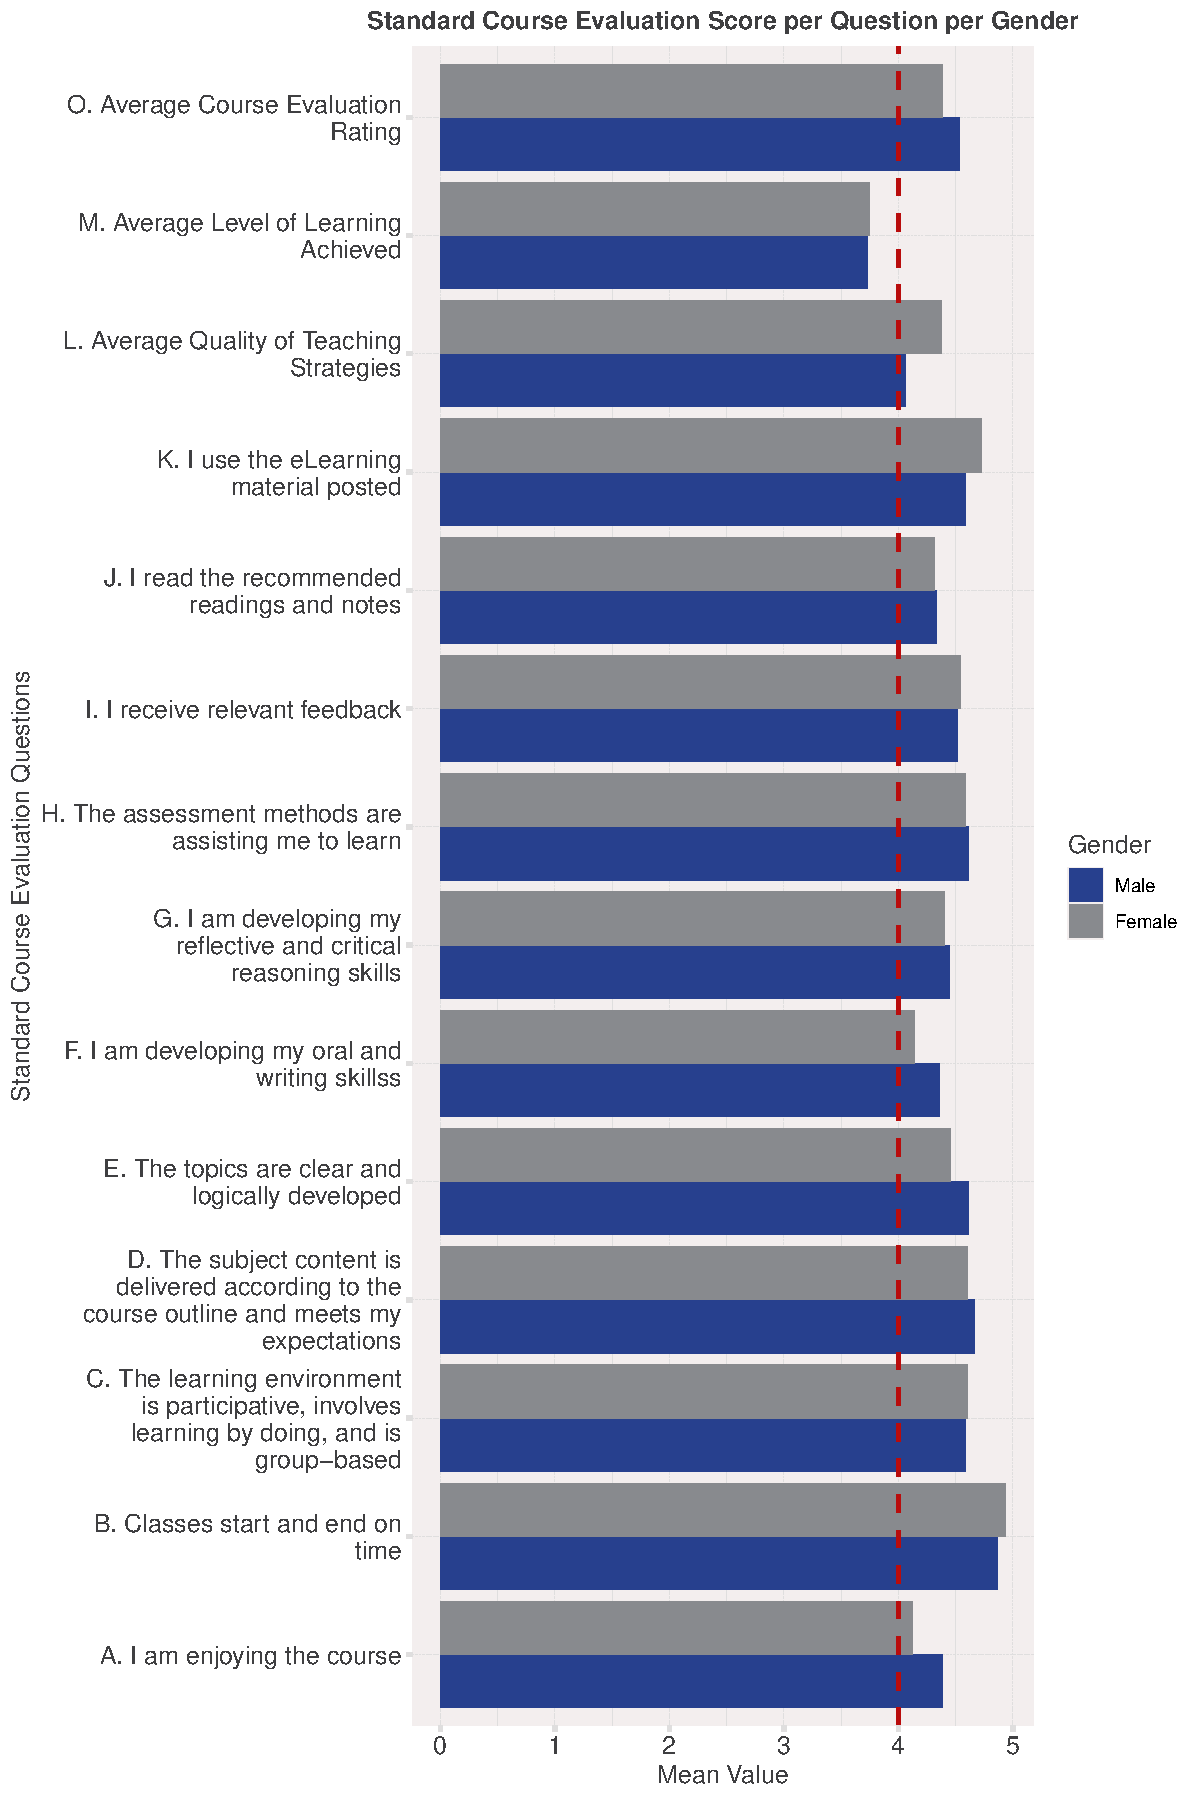
\includegraphics{Mid-SemesterCourseEvaluation-20240819-20241125-ADB-BBIT2.2_files/figure-latex/VisualizationsForCourseEvaluationResultsperGender-1.pdf}

\newpage

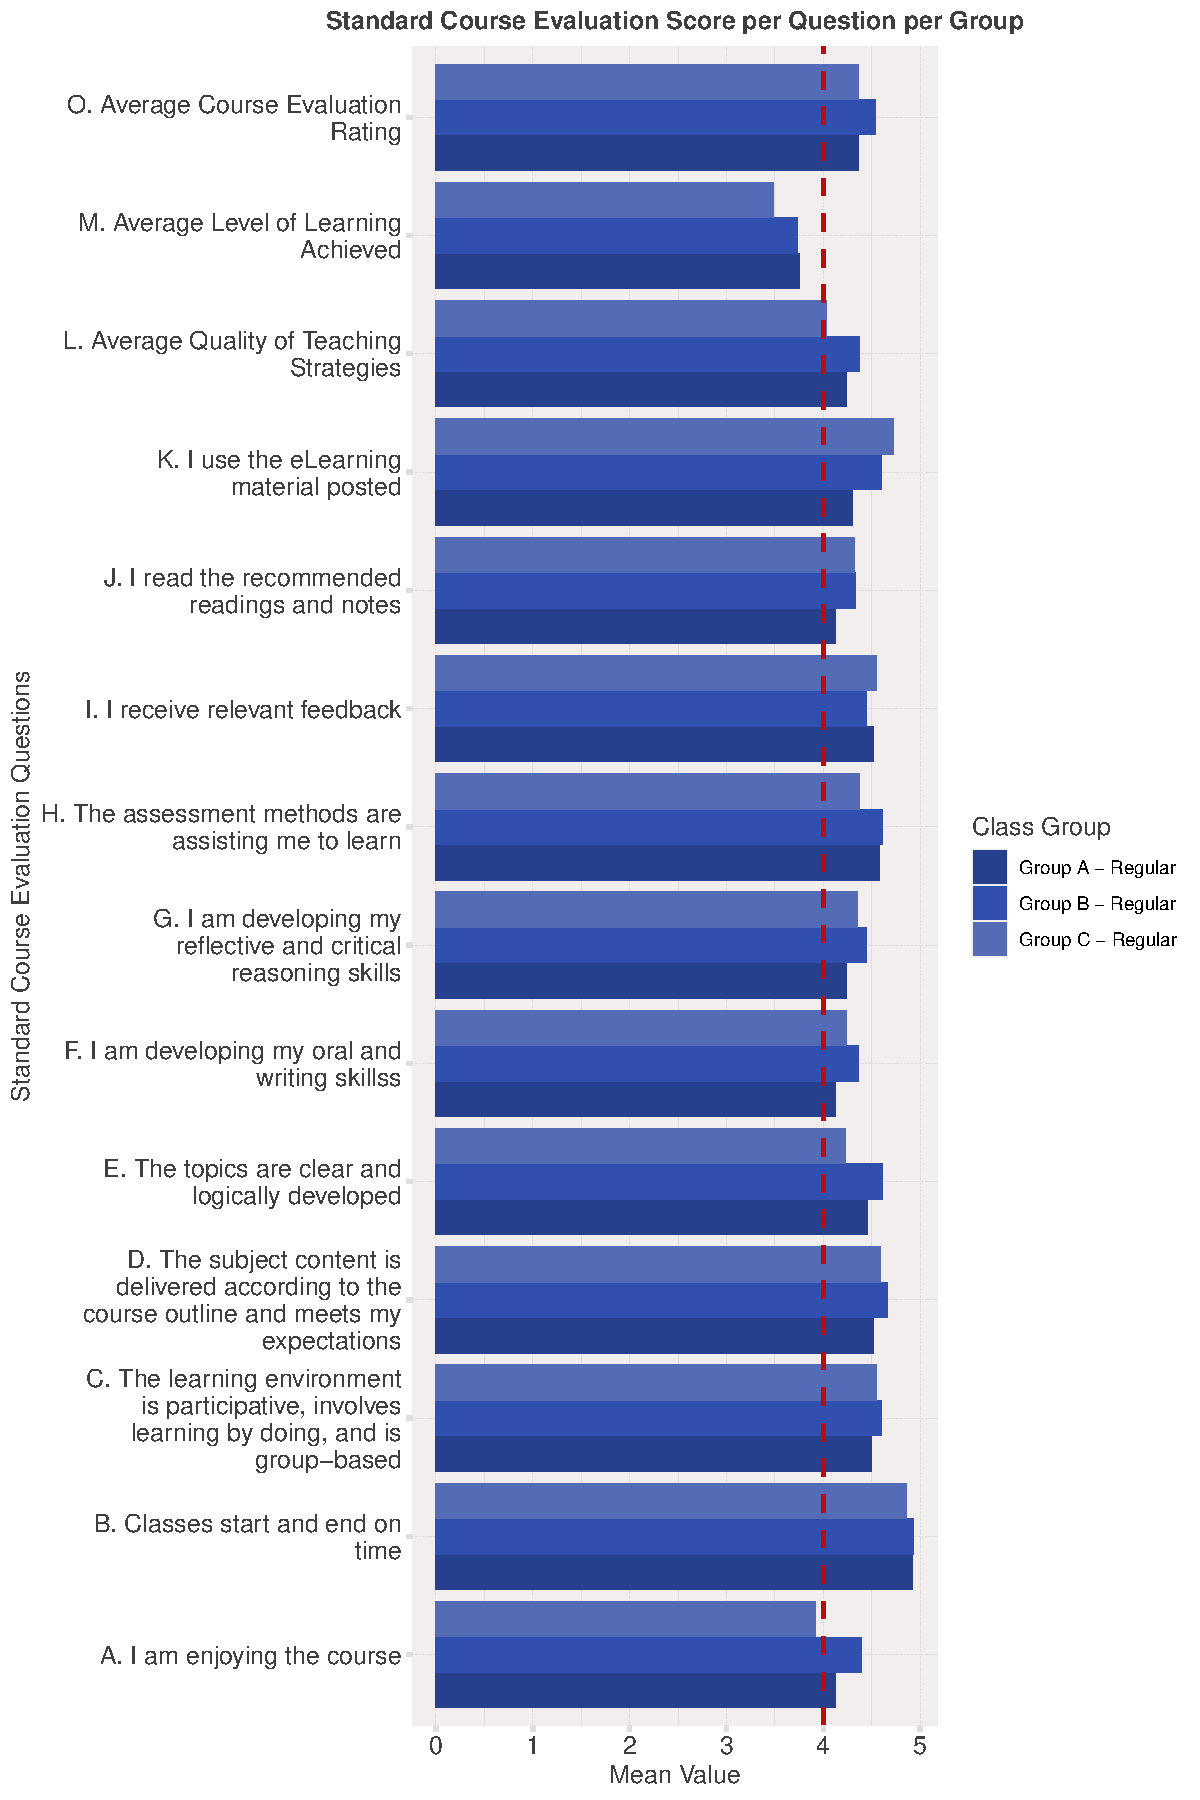
\includegraphics{Mid-SemesterCourseEvaluation-20240819-20241125-ADB-BBIT2.2_files/figure-latex/VisualizationsForCourseEvaluationResultsperGroup-1.pdf}

\newpage

\subsection{Correlations}\label{correlations}

Please refer to \hyperref[appendix-a-full-name-of-variables]{Appendix A:
Full Name of Variables} for the full name of the variables listed in the
correlation plot below.

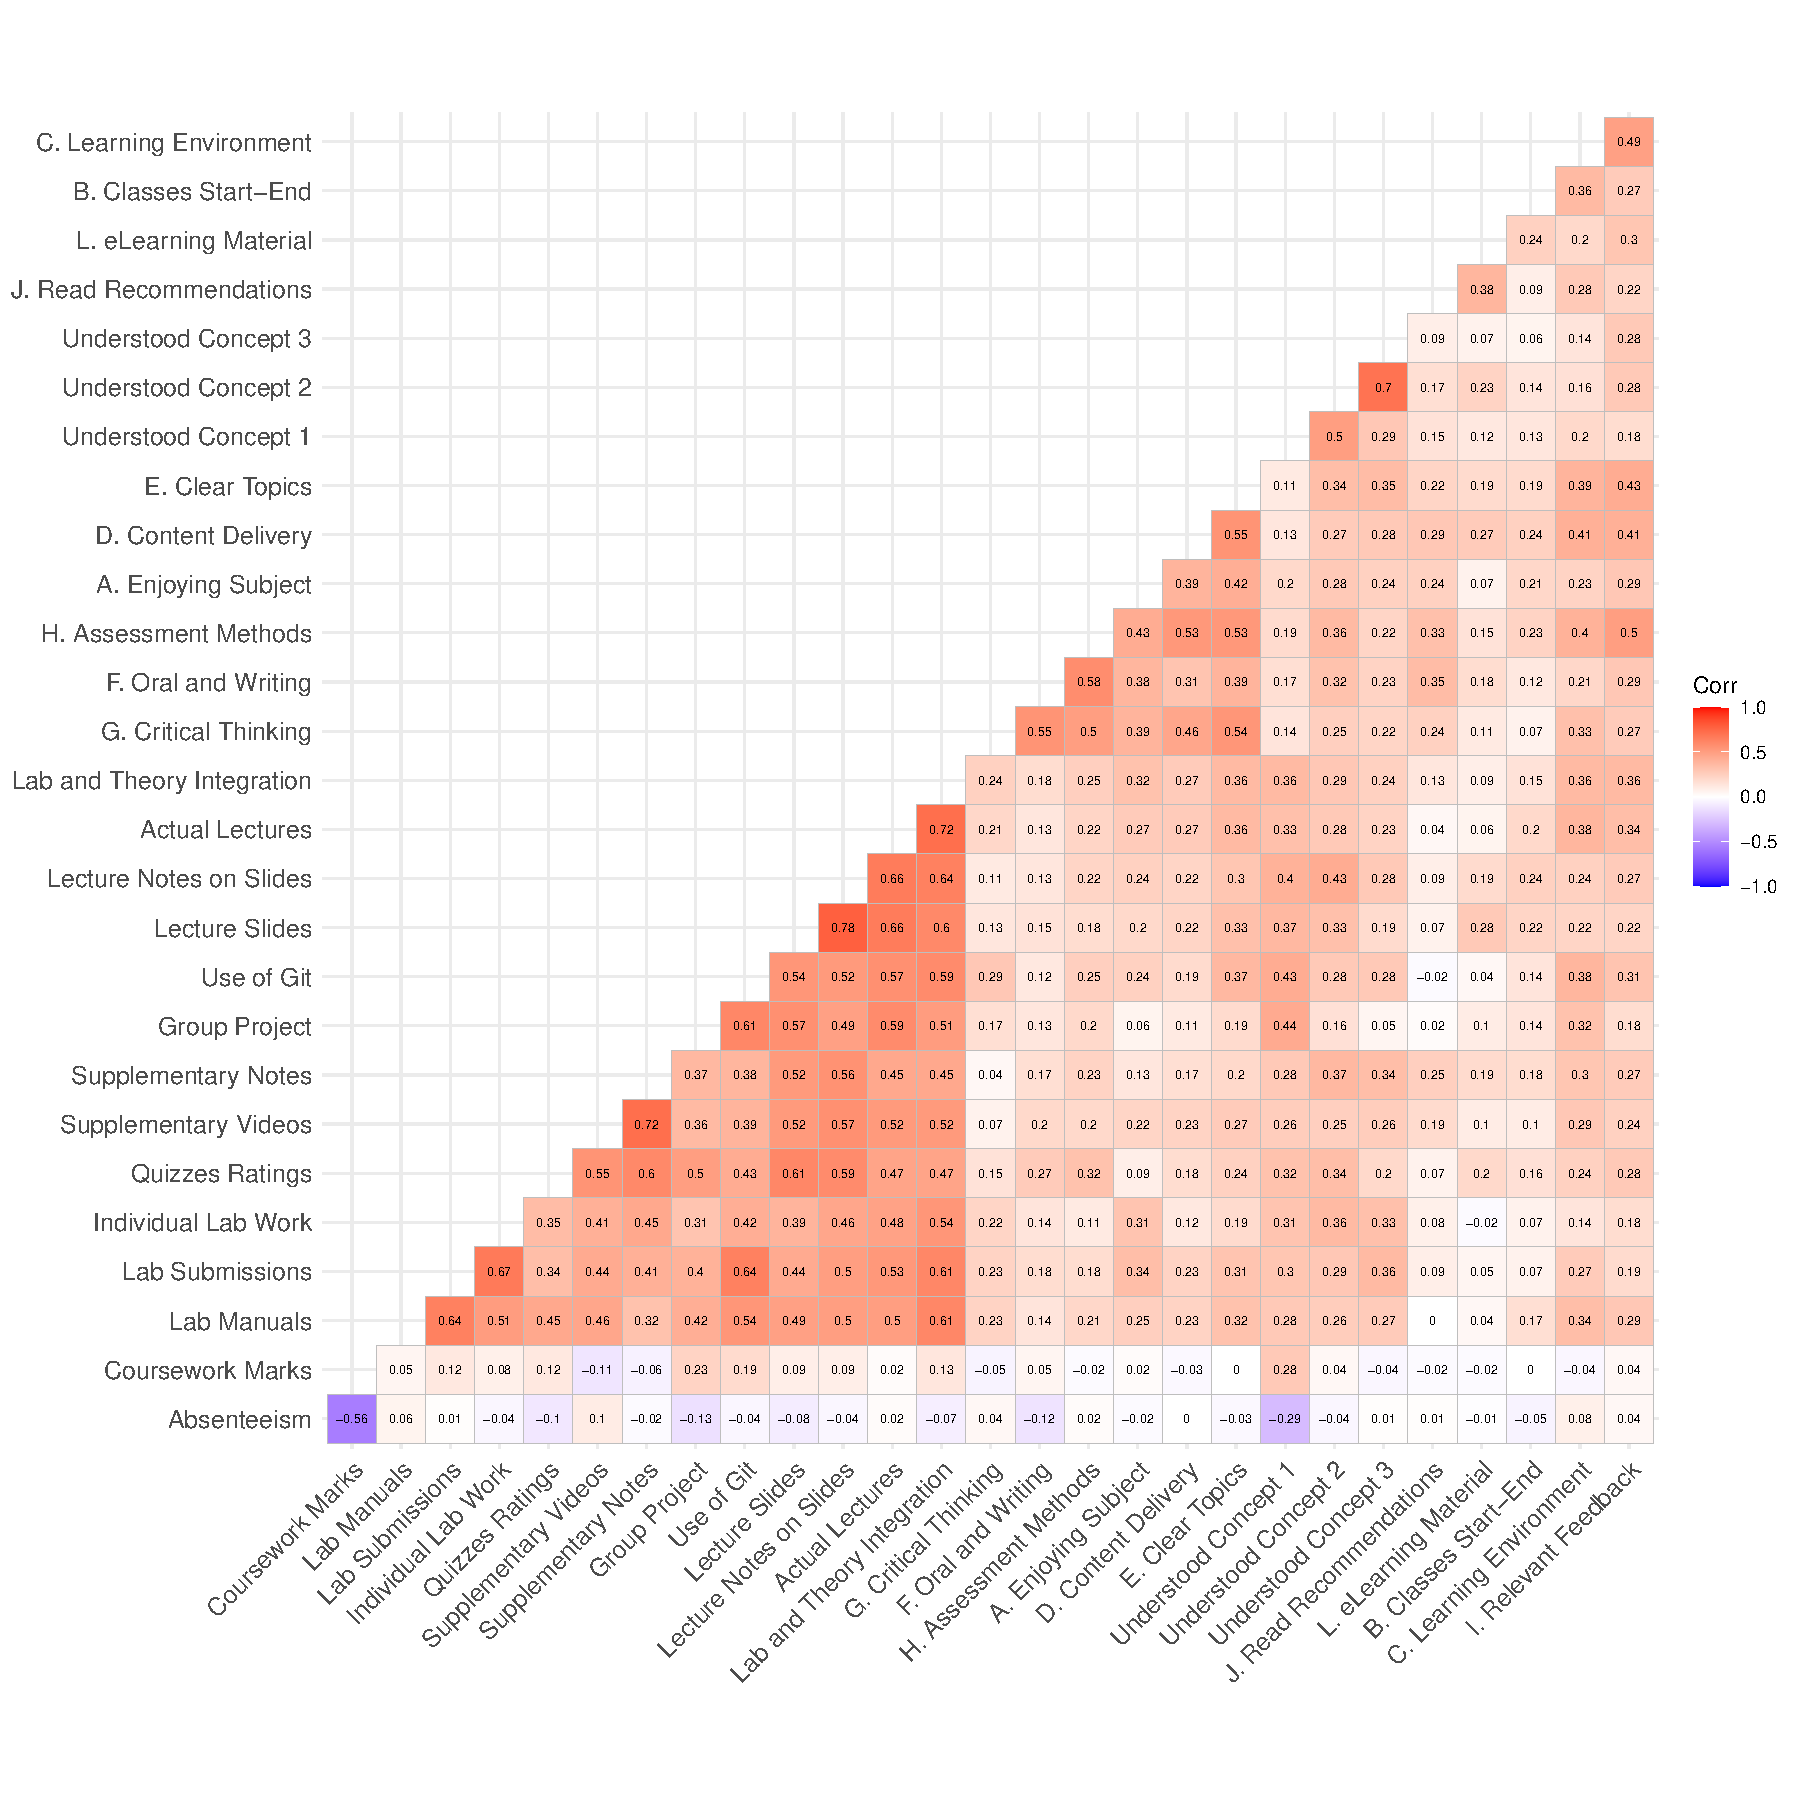
\includegraphics{Mid-SemesterCourseEvaluation-20240819-20241125-ADB-BBIT2.2_files/figure-latex/CorrelationMatrixWithFigures-1.pdf}

\subsubsection{Interesting Correlations}\label{interesting-correlations}

Correlations worth noting include:

\begin{itemize}
\item
  \textbf{0.78 correlation} between ``lectures slides'' and ``lecture
  notes on some of the lecture slides'': \emph{Having lecture notes to
  accompany some lecture slides may improve the overall quality of the
  lecture slide}
\item
  \textbf{0.72 correlation} between ``the quality of the lectures given
  (quality measured by the breadth (the full span of knowledge of a
  subject) and depth (the extent to which specific topics are focused
  upon, amplified, and explored) of learning - NOT quality measured by
  how fun, comical, or entertaining the lectures are)'' and ``the
  integration of practical labs in most classes even if it is not in a
  computer lab'': \emph{Mixing practicals with theory in the same class
  may improve the overall quality of the lecture.}
\item
  \textbf{0.72 correlation} between ``Supplementary videos to watch as
  an additional explanation of a topic'' and ``Supplementary content to
  read'': \emph{Students who find the supplementary videos useful with
  regard to their learning are likely to also find the supplementary
  notes useful}
\item
  \textbf{0.7 correlation} between ``understood Concept 2 (Conceptual
  Data Modelling)'' and ``understood Concept 3 (Database Constraints)'':
  \emph{Most students who do not understand Concept 2 also do not
  understand Concept 3. It may be necessary for students to understand
  Concept 2 before moving on to Concept 3.}
\item
  \textbf{-0.56 correlation} between ``Absenteeism'' and ``Coursework
  Marks'': \emph{It is probable that the higher the absenteeism, the
  lower the student's coursework marks}
\item
  \textbf{-0.29 correlation} between ``Absenteeism'' and ``Understood
  Concept 1'': \emph{It is probable that the more late students are to
  register for the course and begin the semester, the harder it is for
  them to understand concept 1}
\end{itemize}

\newpage

The negative correlation between ``absenteeism'' and ``coursework
marks'' is slightly stronger among the female students, i.e., the more
classes a student misses, the worse their performance, especially for
female students.

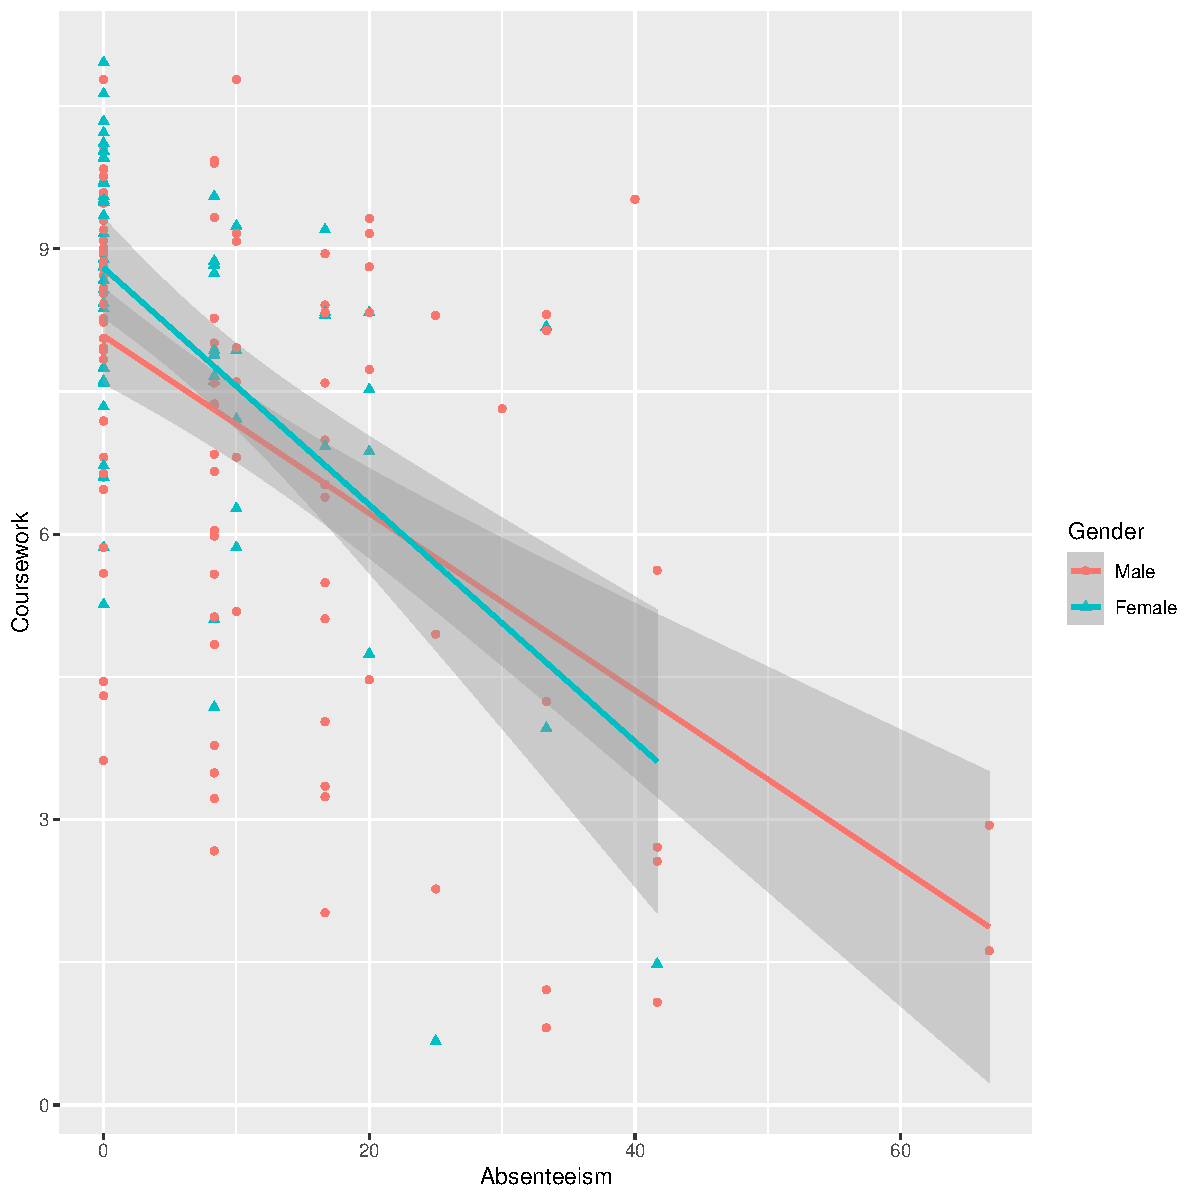
\includegraphics{Mid-SemesterCourseEvaluation-20240819-20241125-ADB-BBIT2.2_files/figure-latex/DrillDownCorr1-1.pdf}

\newpage

\subsubsection{Absenteeism Percentage}\label{absenteeism-percentage}

\paragraph{Absenteeism by Specific Class
Group}\label{absenteeism-by-specific-class-group}

Group C has the lowest absenteeism issues despite having a class on
Friday afternoon.

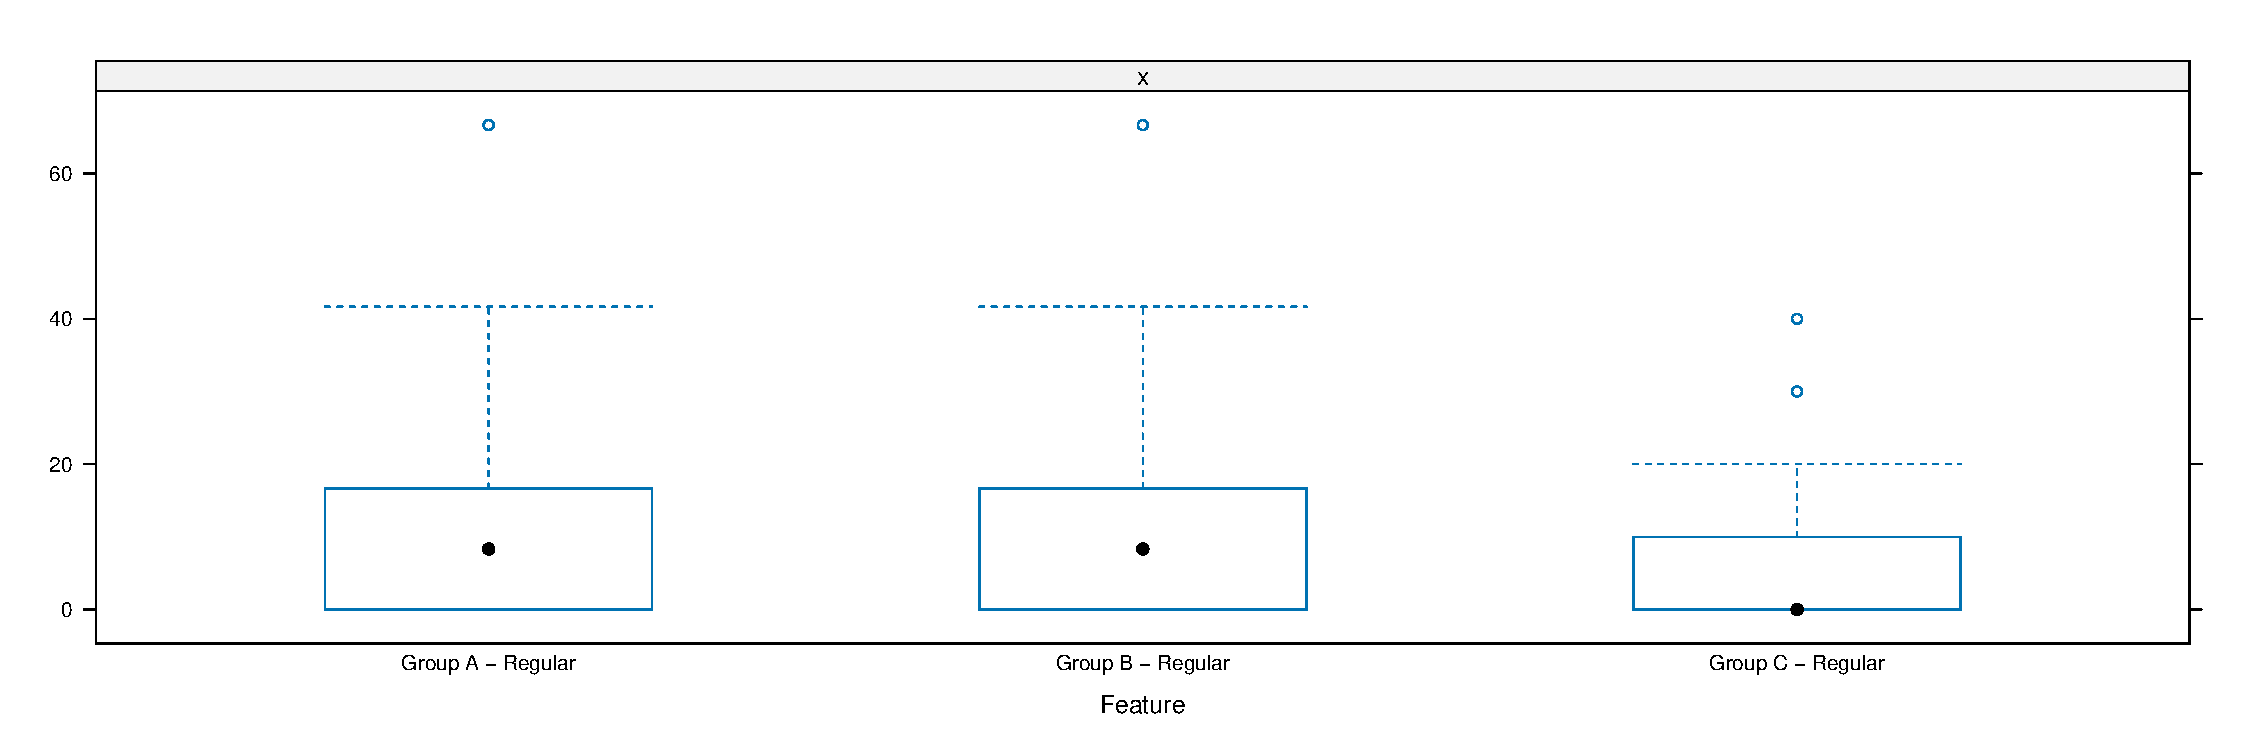
\includegraphics{Mid-SemesterCourseEvaluation-20240819-20241125-ADB-BBIT2.2_files/figure-latex/AbsenteeismBoxandWhiskerSpecificGroup-1.pdf}

\newpage

\paragraph{Absenteeism by Gender}\label{absenteeism-by-gender}

Male students have more absenteeism challenges than female students.

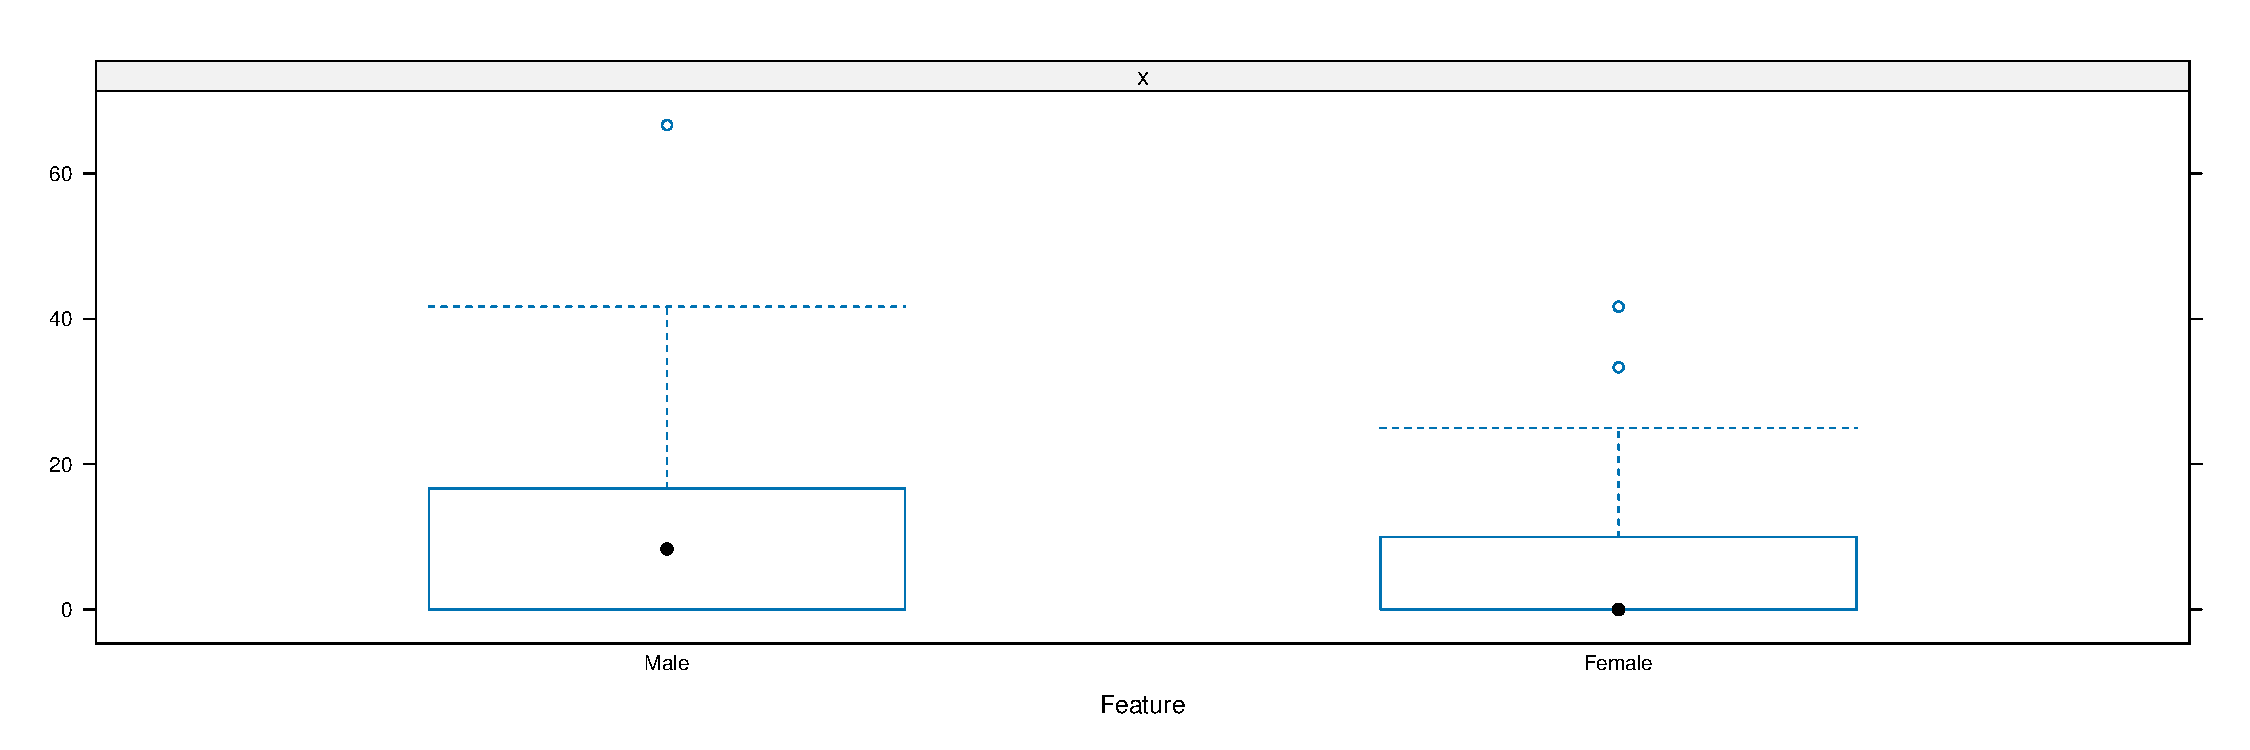
\includegraphics{Mid-SemesterCourseEvaluation-20240819-20241125-ADB-BBIT2.2_files/figure-latex/AbsenteeismBoxandWhiskerGender-1.pdf}

\newpage

\section{Qualitative Data Analysis}\label{qualitative-data-analysis}

\subsection{Sentiment Analysis
(Lexicon-Based)}\label{sentiment-analysis-lexicon-based}

\subsubsection{Chord Diagram of Sentiments for Likes per Class
Group}\label{chord-diagram-of-sentiments-for-likes-per-class-group}

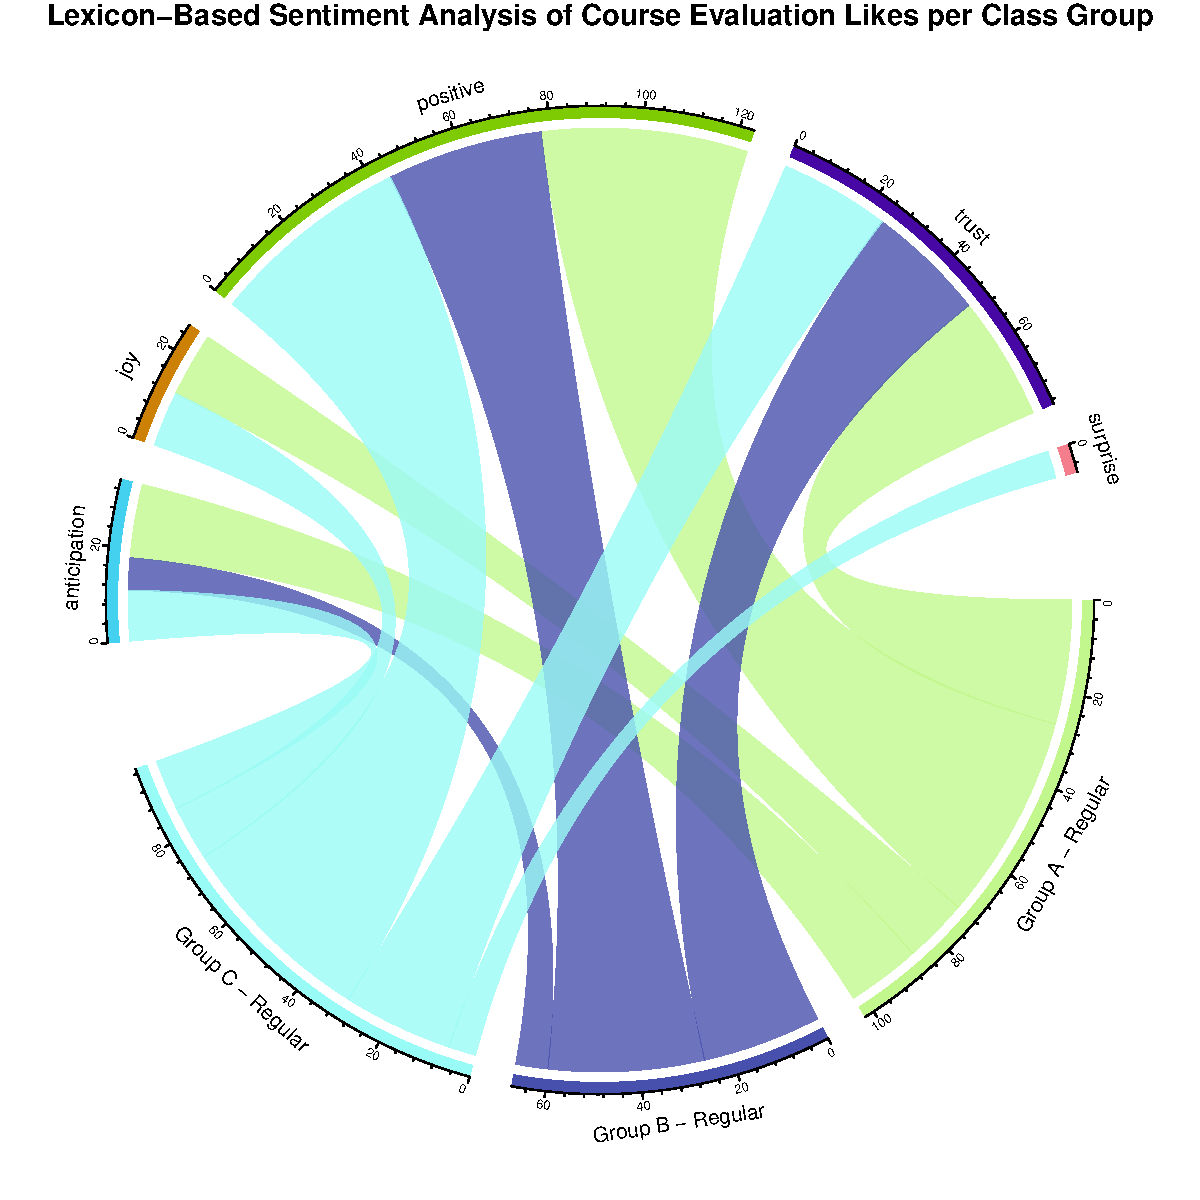
\includegraphics{Mid-SemesterCourseEvaluation-20240819-20241125-ADB-BBIT2.2_files/figure-latex/ChordDiagramLikesPerGroup-1.pdf}

The sentiments expressed based on the choice of words are similar across
all the 3 groups, i.e., positive sentiments.

\newpage

\subsubsection{Chord Diagram of Sentiments for Likes per Class
Gender}\label{chord-diagram-of-sentiments-for-likes-per-class-gender}

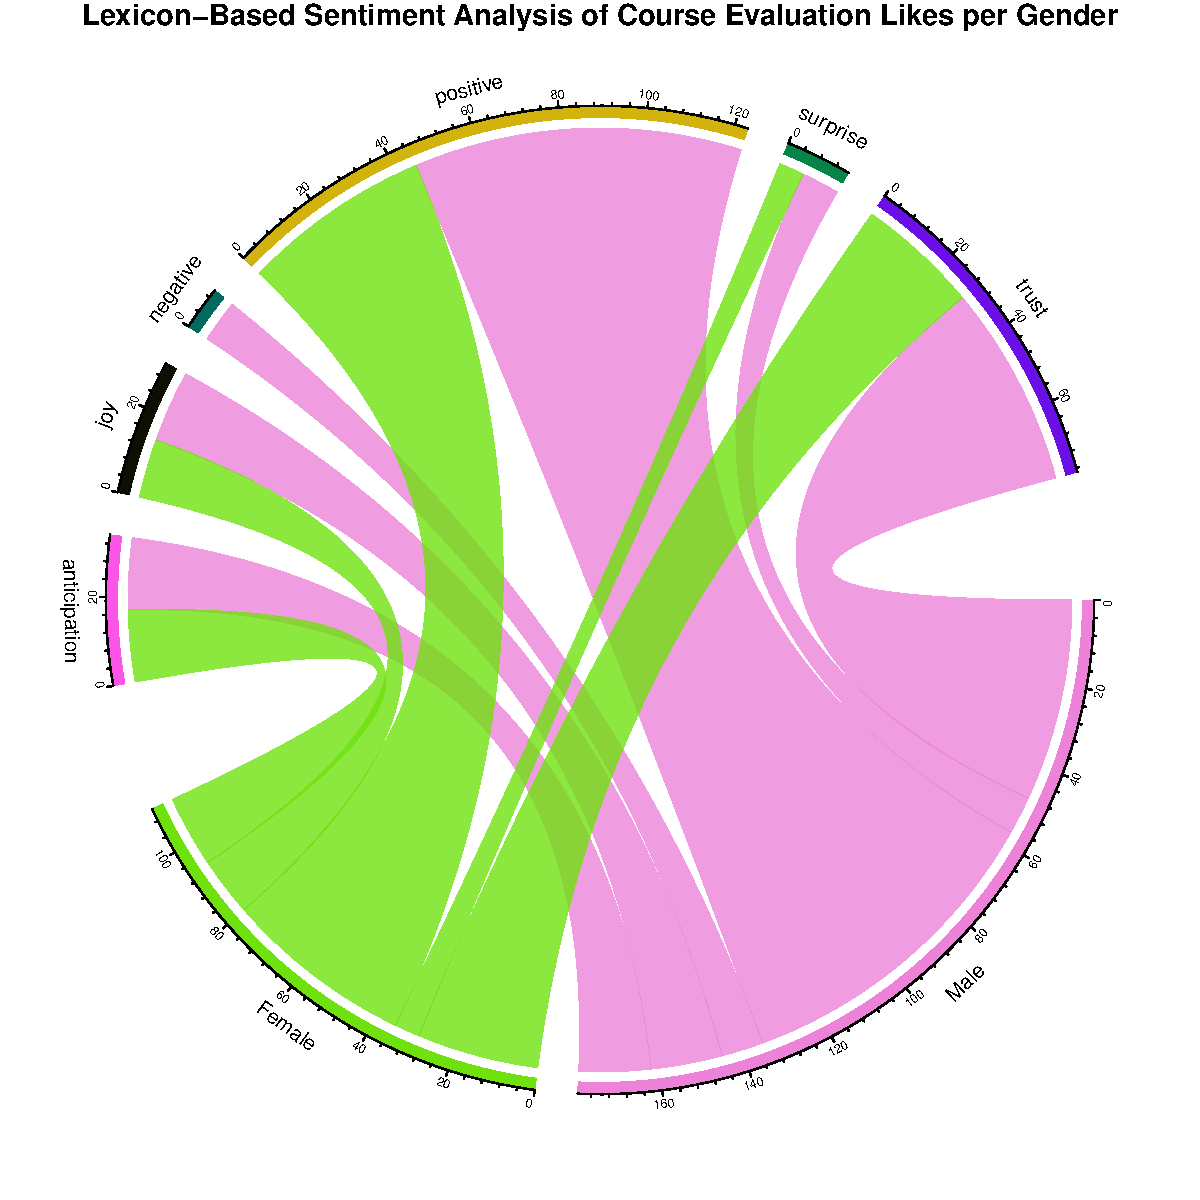
\includegraphics{Mid-SemesterCourseEvaluation-20240819-20241125-ADB-BBIT2.2_files/figure-latex/ChordDiagramLikesPerGender-1.pdf}

The results are similar for both genders but the male students are more
positive and trustworthy based on their choice of words for the ``likes
question''.

\newpage

\subsubsection{Chord Diagram of Sentiments for Wishes per Class
Group}\label{chord-diagram-of-sentiments-for-wishes-per-class-group}

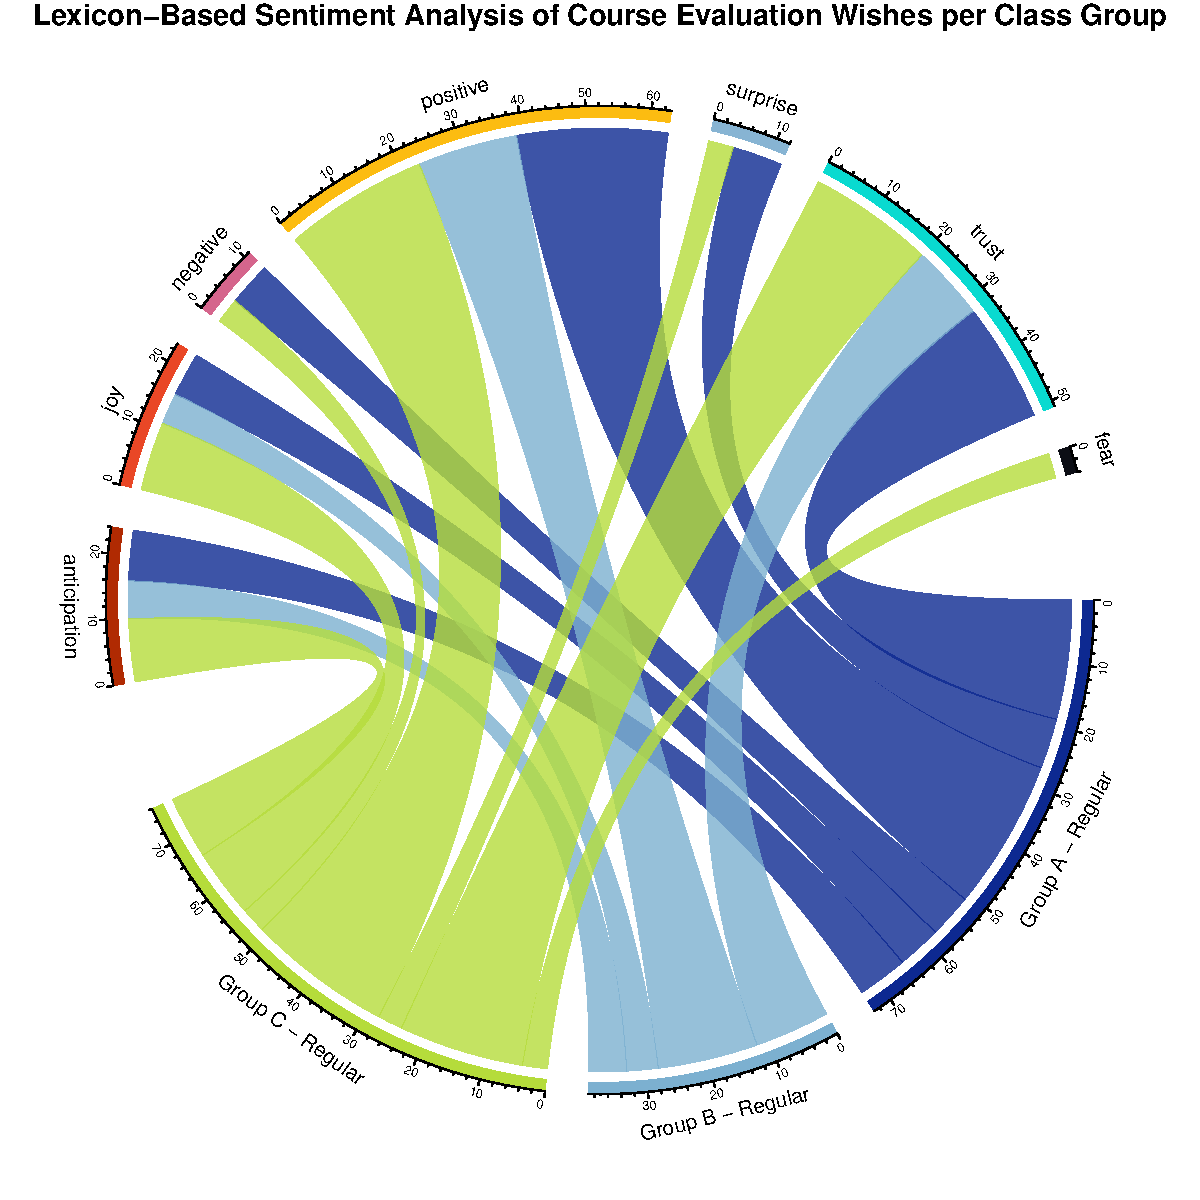
\includegraphics{Mid-SemesterCourseEvaluation-20240819-20241125-ADB-BBIT2.2_files/figure-latex/ChordDiagramPerGroup_Wishes-1.pdf}

Group A and C express more negative sentiments with Group C also
expressing fear based on their choice of words for the ``wishes
question''.

\newpage

\subsubsection{Chord Diagram of Sentiments for Wishes per
Gender}\label{chord-diagram-of-sentiments-for-wishes-per-gender}

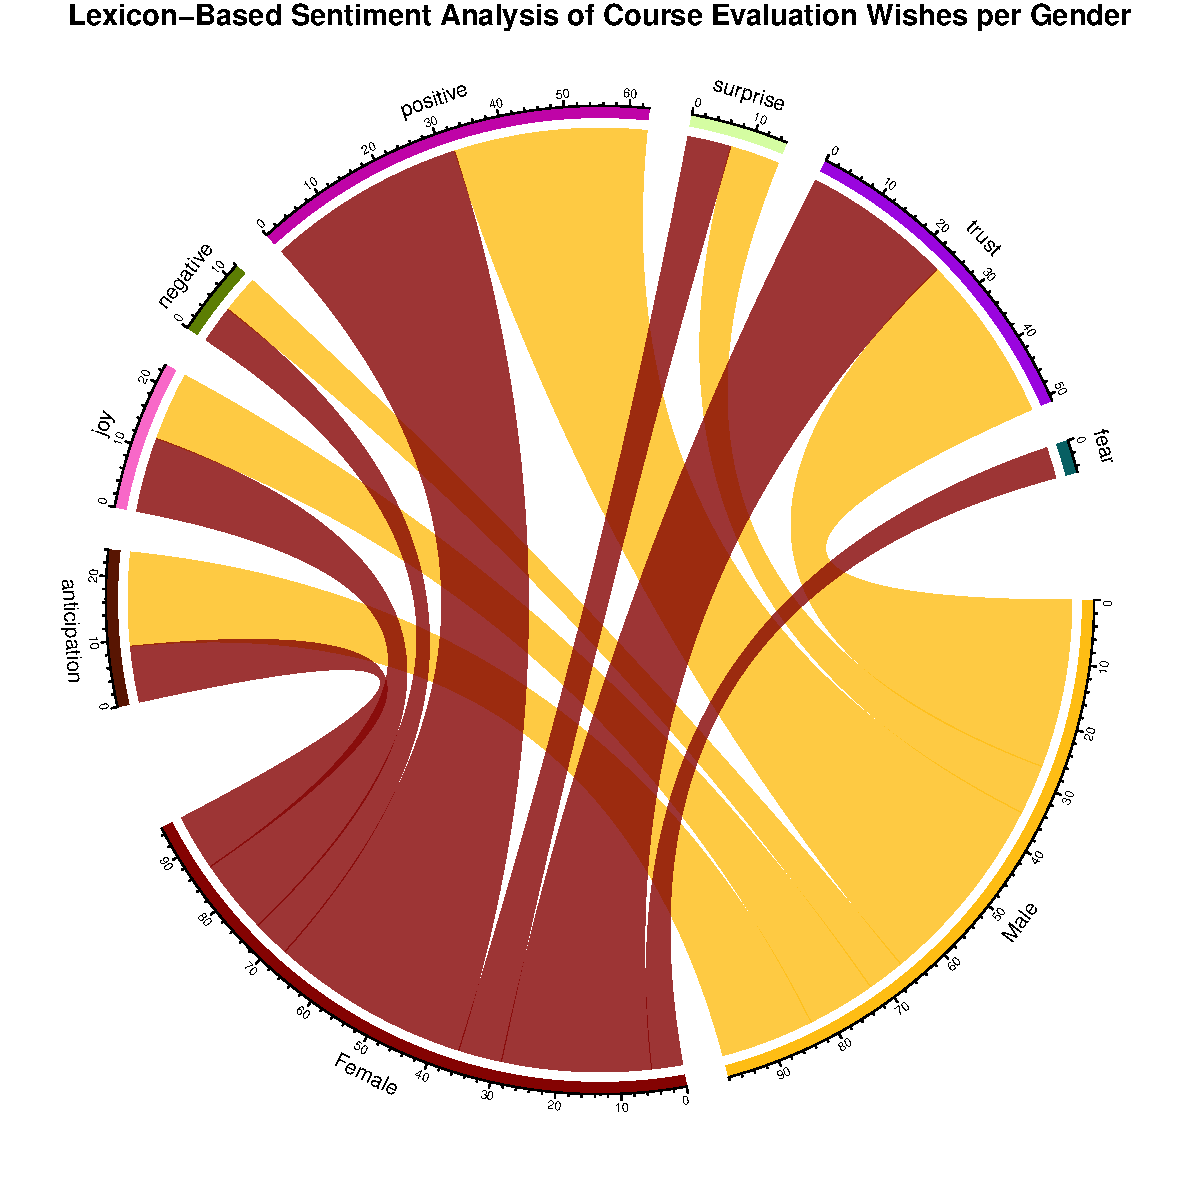
\includegraphics{Mid-SemesterCourseEvaluation-20240819-20241125-ADB-BBIT2.2_files/figure-latex/ChordDiagramPerGender_Wishes-1.pdf}

The sentiments for wishes are similar across both genders but female
students express more fear than male students based on their choice of
words.

\newpage

\subsection{Topic Modelling (Latent Dirichlet Allocation (LDA)
based)}\label{topic-modelling-latent-dirichlet-allocation-lda-based}

The goal of topic modelling is to identify latent (hidden) terms
(topics) in the students' course evaluation textual feedback. In this
case, a topic is a mixture of words and a student's textual feedback is
a combination of one or more topics (mixed-membership model).

The 2 topics for the ``likes'' (as guided by the LDA model) are:

\begin{enumerate}
\def\labelenumi{\arabic{enumi}.}
\item
  Topic 1: Well-Taught for Ease of Understanding
\item
  Topic 2: Practical
\item
  Topic 3: Organized
\end{enumerate}

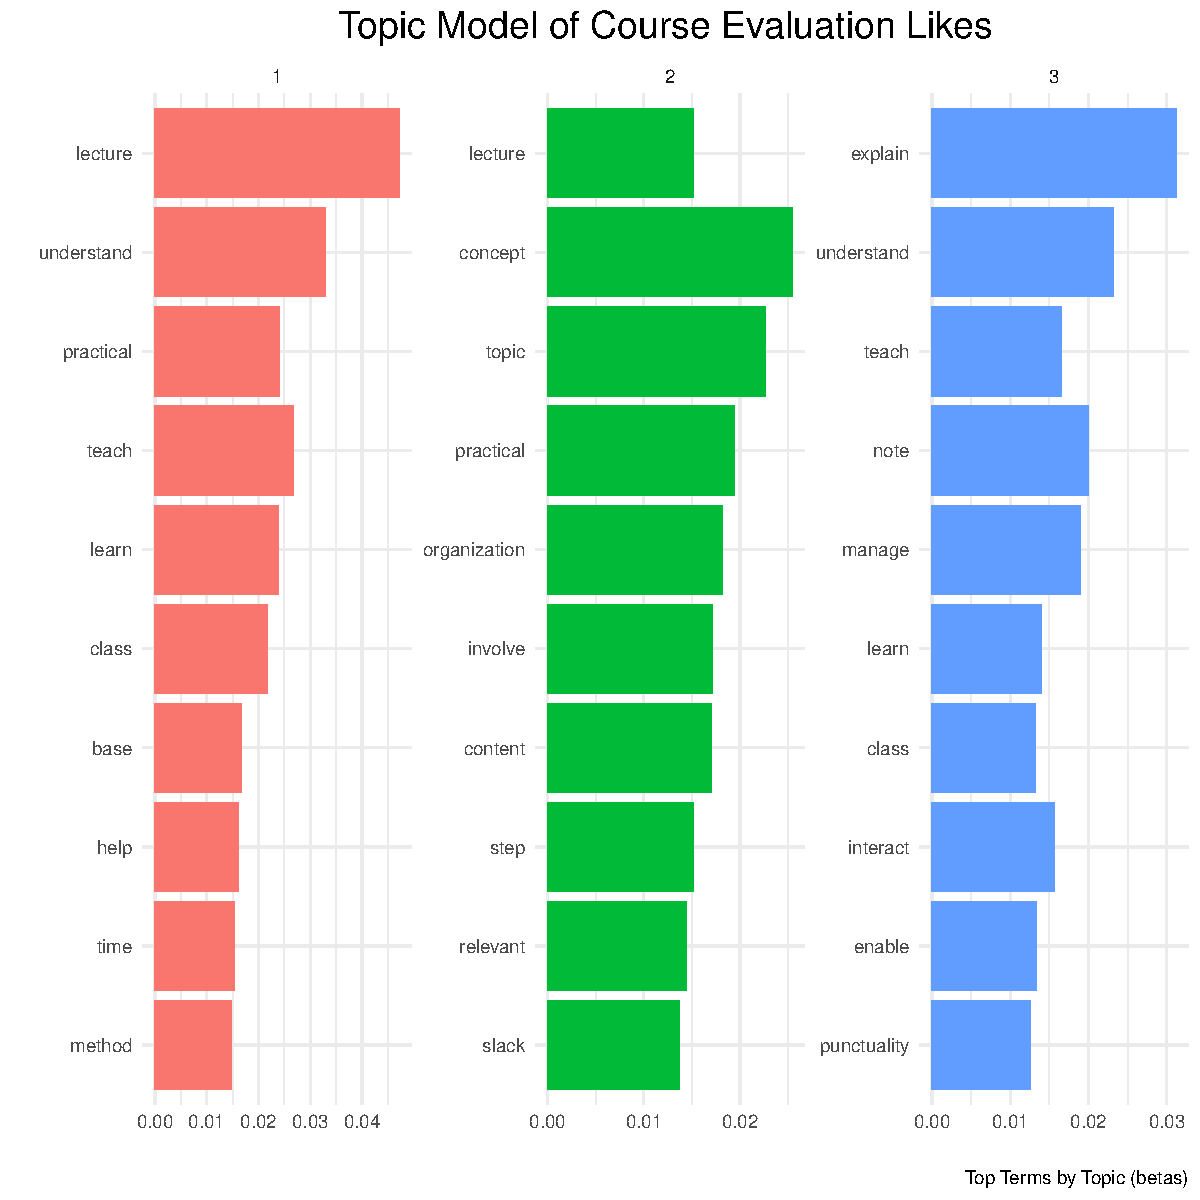
\includegraphics{Mid-SemesterCourseEvaluation-20240819-20241125-ADB-BBIT2.2_files/figure-latex/visualizations_for_likes_topic_modelling-1.pdf}

\newpage

The 5 topics for the ``wishes'' (as guided by the LDA model) are:

\begin{enumerate}
\def\labelenumi{\arabic{enumi}.}
\item
  Topic 1: Extend the deadlines
\item
  Topic 2: Reduce the group work
\item
  Topic 3: More breaks during lectures
\end{enumerate}

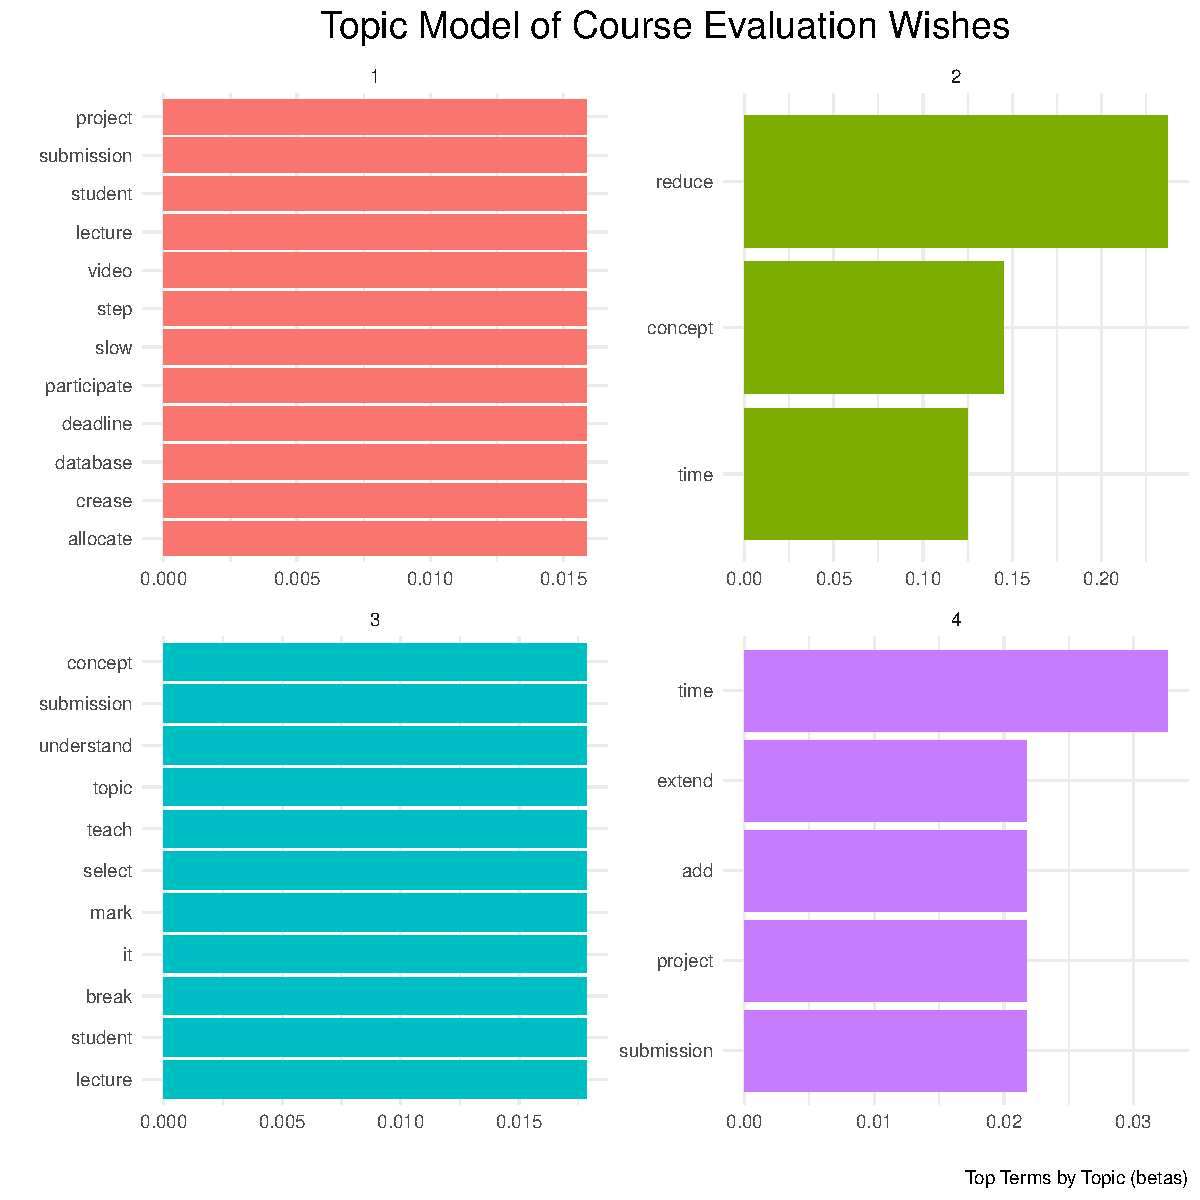
\includegraphics{Mid-SemesterCourseEvaluation-20240819-20241125-ADB-BBIT2.2_files/figure-latex/visualizations_for_wishes_topic_modelling-1.pdf}

\newpage

\section{Appendices}\label{appendices}

\subsection{Appendix A: Full Name of
Variables}\label{appendix-a-full-name-of-variables}

The following variables have been renamed to fit the correlation plots:

\begin{verbatim}
`A. Enjoying Subject` = `B - 1. I am enjoying the course`,
`B. Classes Start-End` = `B - 2. Classes start and end on time`,
`C. Learning Environment` = `B - 3. The learning environment is participative, involves learning by doing, and is group-based`,
`D. Content Delivery` = `B - 4. The subject content is delivered according to the course outline and meets my expectations`,
`E. Clear Topics` = `B - 5. The topics are clear and logically developed`,
 `F. Oral and Writing` = `B - 6. I am developing my oral and writing skills`,
`G. Critical Thinking` = `B - 7. I am developing my reflective and critical reasoning skills`,
 `H. Assessment Methods` = `B - 8. The assessment methods are assisting me to learn`,
`I. Relevant Feedback` = `B - 9. I receive relevant feedback`,
`J. Read Recommendations` = `B - 10. I read the recommended readings and notes`,
`L. eLearning Material` = `B - 11. I use the eLearning material posted`,

`Understood Concept 1` = `C - 1. Concept 1 of 6: Business Processes`,
`Understood Concept 2` = `C - 2. Concept 2 of 6: Conceptual Data Modelling`,
`Understood Concept 3` = `C - 3. Concept 3 of 6: Database Constraints`,

`Group Project` = `D - 1. The group project`,
`Quizzes Ratings` = `D - 2. Quizzes at the end of each concept`,
`Lab Manuals` = `D - 3. Lab manuals that outline the steps to follow during the labs`,
`Lab Submissions` = `D - 4. Required lab work submissions at the end of each lab manual that outline the activity to be done on your own`,
`Use of Git` = `D - 5. Labs that require you to use Git to work in a team`,
`Individual Lab Work` = `D - 6. Labs that require you to work alone`,
`Supplementary Videos` = `D - 7. Supplementary videos to watch as an additional explanation of a topic`,
`Supplementary Notes` = `D - 8. Supplementary content to read`,
`Lecture Slides` = `D - 9. Lectures slides`,
`Lecture Notes on Slides` = `D - 10. Lecture notes on some of the lecture slides`,
`Actual Lectures` = `D - 11. The quality of the lectures given (quality measured by the breadth (the full span of knowledge of a subject) and depth (the extent to which specific topics are focused upon, amplified, and explored) of learning - NOT quality measured by how fun, comical, or entertaining the lectures are)`,
`Lab and Theory Integration` = `D - 12. The integration of practical labs in most classes even if it is not in a computer lab`,

`Coursework Marks` = `Coursework`
\end{verbatim}

\newpage

\subsection{Appendix B: Raw Qualitative
Data}\label{appendix-b-raw-qualitative-data}

\subsubsection{Likes}\label{likes}

The raw data of the likes is as follows:

\begin{verbatim}
##   [1] "Class punctuality\nCommunity feedback on Slack"                                                                                                                                                                                                   
##   [2] "I love that we have labs that enable me to engage with the content and get some experience of what I would be needed to do in the work environment."                                                                                              
##   [3] "N/A"                                                                                                                                                                                                                                              
##   [4] "The content delivery is well done"                                                                                                                                                                                                                
##   [5] "-"                                                                                                                                                                                                                                                
##   [6] "I like the learning pace and the content with the labs is executable"                                                                                                                                                                             
##   [7] "The topics \nLabs and group work"                                                                                                                                                                                                                 
##   [8] "The delivery\nThe content"                                                                                                                                                                                                                        
##   [9] "The quizzes, how we learned to use new software i.e. Slack"                                                                                                                                                                                       
##  [10] "Inclusive learning\nrelevant feedback is given"                                                                                                                                                                                                   
##  [11] "Coding in vs and applying it in GitHub"                                                                                                                                                                                                           
##  [12] "None"                                                                                                                                                                                                                                             
##  [13] "n/a"                                                                                                                                                                                                                                              
##  [14] "Null"                                                                                                                                                                                                                                             
##  [15] "I like how we are given a quiz after each concept in this unit.\nIn this unit, I also like the way we already have all the content online for the whole semester."                                                                                
##  [16] "The learning is very enjoyable and interesting"                                                                                                                                                                                                   
##  [17] "I like the concept of doing the short quizzes on google classroom"                                                                                                                                                                                
##  [18] "Triggers \nand also capabilities and constraints"                                                                                                                                                                                                 
##  [19] "Lessons are interesting and push us to get more knowledge and to do better"                                                                                                                                                                       
##  [20] "It is Fun. It is interactive"                                                                                                                                                                                                                     
##  [21] "1. I enjoy how organized the results are so I am able to track my performance from the start to the finish \n2. I like how detailed the lab manuals are because I am able to fully understand what is happening"                                  
##  [22] "its interesting. its relevant"                                                                                                                                                                                                                    
##  [23] "I like that it is much more practical as performing activities is much more beneficial that just sitting an having the information exposited, I also like that the steps for the practicals are detailed and give explanations on their functions"
##  [24] "I like that the lecturer gives feedback regarding the projects and labs and that the classes start on time\n"                                                                                                                                     
##  [25] "The lecturer has great delivery method and tries to be at per with his class\nThe lecturer  takes his work seriously and gives his students clear expectations"                                                                                   
##  [26] "The class is quite interactive and teamwork is also shown in class"                                                                                                                                                                               
##  [27] "the quizes  given\nthe way the content is delivered"                                                                                                                                                                                              
##  [28] "I like how informative the unit is.\nI like how there is time allocated to work with my peers, it allows me to understand  the concepts more."                                                                                                    
##  [29] "The lecturer explains things well,the lec goes with a good pace"                                                                                                                                                                                  
##  [30] "configuration of a database transaction\nevent scheduling"                                                                                                                                                                                        
##  [31] "Its interactive"                                                                                                                                                                                                                                  
##  [32] "interactiveness and time keeping"                                                                                                                                                                                                                 
##  [33] "Assistance when someone has issues during labworks\nThe step by step procedures to do the labs"                                                                                                                                                   
##  [34] "Broading my knowledge and unnderstanding\n"                                                                                                                                                                                                       
##  [35] "1.The quizzes\n2.The project"                                                                                                                                                                                                                     
##  [36] "The timely response on slack\nThe quizzes after each concept"                                                                                                                                                                                     
##  [37] "The delivery of the content,the lecturer's commitment on assisting a peson individually"                                                                                                                                                          
##  [38] "#NAME?"                                                                                                                                                                                                                                           
##  [39] "#NAME?"                                                                                                                                                                                                                                           
##  [40] "the topics are taught well , One is guided and what and how they are supposed to do the exercises"                                                                                                                                                
##  [41] "OK"                                                                                                                                                                                                                                               
##  [42] "1. The lecturer takes his time to explain concepts \n2. The lab manuals are well laid out"                                                                                                                                                        
##  [43] "The quiz\nThe project"                                                                                                                                                                                                                            
##  [44] "topic one and two"                                                                                                                                                                                                                                
##  [45] "The group work makes it fun and engaging\nThe lecturer manages time well, classes end in good time"                                                                                                                                               
##  [46] "The group project\nThe way everything is organized"                                                                                                                                                                                               
##  [47] "Its good that you keep pushing us .... Thats what amazes me in this unit"                                                                                                                                                                         
##  [48] "Content delivery\nQuizes"                                                                                                                                                                                                                         
##  [49] "It is very organized, the assignments, labs and group work\nThe concepts are understandable\n"                                                                                                                                                    
##  [50] "Explaining being explained in steps by the lecturer.\n"                                                                                                                                                                                           
##  [51] "Learning new things.\nWe do most of the work ourselves so we learn while practicing"                                                                                                                                                              
##  [52] "Lecturer explains everything to the tea"                                                                                                                                                                                                          
##  [53] "."                                                                                                                                                                                                                                                
##  [54] "The lecturer is always punctual\nThe learning is efficient"                                                                                                                                                                                       
##  [55] "Lecturer"                                                                                                                                                                                                                                         
##  [56] "Fun"                                                                                                                                                                                                                                              
##  [57] "1. I like it \n2.Good lectures"                                                                                                                                                                                                                   
##  [58] "It is very interactive and fun \nI get to learn new skills based on different perspectives"                                                                                                                                                       
##  [59] "1.Very well explained\n2.Interesting"                                                                                                                                                                                                             
##  [60] "It is very practical\nFeedback is relevant and on time"                                                                                                                                                                                           
##  [61] "The practicals\nThe teamwork"                                                                                                                                                                                                                     
##  [62] "the detailed explained slides and the time taken to make sure everyone understands"                                                                                                                                                               
##  [63] "The unit is really involving which is good \nThe unit is interesting"                                                                                                                                                                             
##  [64] "The clear outline of the work\nThe practical examples"                                                                                                                                                                                            
##  [65] "The applicability of the unit in modern world"                                                                                                                                                                                                    
##  [66] "I like the labs and quizzes which check on our progress"                                                                                                                                                                                          
##  [67] "I like how the lecturer explains the concepts clearly and logically\nI like the fact that the lec is always ready to explain unclear and ambiguous concepts"                                                                                      
##  [68] "Well Organised, Interactive"                                                                                                                                                                                                                      
##  [69] "The lecturer and what is being taught"                                                                                                                                                                                                            
##  [70] "Use of real world examples. \nAnd Use of structured design and logical thinking"                                                                                                                                                                  
##  [71] "Learning new skills\nLearning problem solving"                                                                                                                                                                                                    
##  [72] "Practice is very important for the long run, Database is very broad"                                                                                                                                                                              
##  [73] "The explanation is simple and easy for me to understand.\nThe class is involving by asking questions"                                                                                                                                             
##  [74] "it is mostly practical"                                                                                                                                                                                                                           
##  [75] "the lab exercises are engaging if one is committed to them.\n\nthe extensive use of the GitHub repositories and the other database tools are equipping with practical database experiences"                                                       
##  [76] "Simple"                                                                                                                                                                                                                                           
##  [77] "-"                                                                                                                                                                                                                                                
##  [78] "i.) Classes start and end on time\nii.) Lab practiclals are interractive and are fun to do"                                                                                                                                                       
##  [79] "The topics are well explained and to one's understanding and learning the topics are interesting as compared to labs"                                                                                                                             
##  [80] "I like the clarity that is offered and the avaliability of the lecturer"                                                                                                                                                                          
##  [81] "He is very organised\nHe is patient when it comes to explaining"                                                                                                                                                                                  
##  [82] "simplified mode of teaching\nproper organization of content"                                                                                                                                                                                      
##  [83] "1. Well organized work plan\n2. Good amount of work load given"                                                                                                                                                                                   
##  [84] "It is very practical and well detailed"                                                                                                                                                                                                           
##  [85] "the quizzes that are given out after each concept are really helpful"                                                                                                                                                                             
##  [86] "Everything is well outlined and oranised\nhe explains the concepts in a good way"                                                                                                                                                                 
##  [87] "How the lecturer organises his work so its easy to find the material that you need"                                                                                                                                                               
##  [88] "The practical interaction with the content\nThe methods of checking content retention"                                                                                                                                                            
##  [89] "The organisation of the lecturers materials \nThe feedback given and the ability to track progress"                                                                                                                                               
##  [90] "It is giving me more ideas and knowledge \nIt is helping in my oral skills"                                                                                                                                                                       
##  [91] "The way the concept is taught with like the examples that are understandable"                                                                                                                                                                     
##  [92] "The quizes offered really help in summarising the topic \nThe lab work manual is simple and easy to follow"                                                                                                                                       
##  [93] "The group work given by the lecturer helps in my understanding of the concept better\nThe quizzes done after every concept which helps me in reminding myself on the concept"                                                                     
##  [94] "1. The lecturer is very organized and teaches the content well.\n2. Resources and materials required to take on this unit are readily available."                                                                                                 
##  [95] "The group gave me idea on how to apply the concepts in real life"                                                                                                                                                                                 
##  [96] "The hands-on practicals.\nThe lab manuals."                                                                                                                                                                                                       
##  [97] "I like the lecturere...He is wonderful and fair"                                                                                                                                                                                                  
##  [98] "I like the practical aspect of the unit \nI like how we explore different aspects of the database"                                                                                                                                                
##  [99] "1. I enjoy the content and lectures in general\n2. I like the labs and the manuals are helpful for understanding"                                                                                                                                 
## [100] "the ability to engage in critical thinking and group participation"                                                                                                                                                                               
## [101] "group work and the quizes"                                                                                                                                                                                                                        
## [102] "The teacher know how to explain the theory parts"                                                                                                                                                                                                 
## [103] "I like the amount of group work that we're given because during the undertaking of the work, I get to learn new concepts.\nWatching supplementary videos online. Some of the videos explain the content in a simpler way."                        
## [104] "Topics well developed\nAble to ask questions freely"                                                                                                                                                                                              
## [105] "The lecturer's teaching style is interactive"                                                                                                                                                                                                     
## [106] "It is well explained \nLecture tutors well"                                                                                                                                                                                                       
## [107] "We are first taught then we do practically which is really helpful \nThe lecturer responds to those who have not understood.He takes time to teach certain concepts"                                                                              
## [108] "It’s engaging and the lab works make it much more interesting. In the few past weeks, I’ve learned a lot more than I learned in the past semester."                                                                                               
## [109] "Helps in thinking critically about data management. Additionally the collaborative projects foster teamwork and problem solving skills."                                                                                                          
## [110] "The group work"                                                                                                                                                                                                                                   
## [111] "I like the organization"                                                                                                                                                                                                                          
## [112] "Mode of delivery,"                                                                                                                                                                                                                                
## [113] "It's good"                                                                                                                                                                                                                                        
## [114] "It's engaging \nIt is practical hence keeping you on your toes"                                                                                                                                                                                   
## [115] "I am able to solve real world problems\nI am able to logically think"                                                                                                                                                                             
## [116] "#NAME?"                                                                                                                                                                                                                                           
## [117] "The lecturer ensures that he has expounded on the topic of the day\nThe lecturer asks questions that engage the class"                                                                                                                            
## [118] "The lecturer explains the concepts in detail before the lab exercises.\nThe lecturer is ready to help whenever a challenge arises when doing the lab manuals in class."                                                                           
## [119] "The group work concept\nThe lecture is always ready to explain a concept you’ve not understood"                                                                                                                                                   
## [120] "1. The teaching methods the lecture always make sure that every student has understood.2. The learning environment ."                                                                                                                             
## [121] "I'm enjoying the unit so far"                                                                                                                                                                                                                     
## [122] "The lab works are educative and creates innovativion"                                                                                                                                                                                             
## [123] "how it is interactive \nthe group work"                                                                                                                                                                                                           
## [124] "It is very practical so it really helps with hands on skills\nContent is clearly broken down and understandable"                                                                                                                                  
## [125] "the topics are well detailed, explanation is well given"                                                                                                                                                                                          
## [126] "It is mostly practical."                                                                                                                                                                                                                          
## [127] "It requires me to be more active and keen"                                                                                                                                                                                                        
## [128] "The lec\nThe content"                                                                                                                                                                                                                             
## [129] "very interesting"                                                                                                                                                                                                                                 
## [130] "Many quizzes help understand"                                                                                                                                                                                                                     
## [131] "The notes are comprehensive and the methods of evaluation are effective"                                                                                                                                                                          
## [132] "practically done"                                                                                                                                                                                                                                 
## [133] "1: It has group based activities.\n2: Some business concepts are involved."                                                                                                                                                                       
## [134] "Teaching methods\nVenue"                                                                                                                                                                                                                          
## [135] "Classes start and end on time"                                                                                                                                                                                                                    
## [136] "Well organized, clear explanations"                                                                                                                                                                                                               
## [137] "1.Good lectures\n2.Friendly lecturer"                                                                                                                                                                                                             
## [138] "The Lecturer is considerate(available for consultation and what not)\n"                                                                                                                                                                           
## [139] "The lecturer involves students in answering questions during lectures which keeps them attentive \nThe lectures are light and easy to understand making them enjoyable"                                                                           
## [140] "The quizzes at the end of each concept help me to remember things \nThe group work is really helpful"                                                                                                                                             
## [141] "1. It is easy to understand.\n2. It enables me to earn more marks in coursework."                                                                                                                                                                 
## [142] "course delivery materials and the lecturer is organized"                                                                                                                                                                                          
## [143] "I like how time is kept"                                                                                                                                                                                                                          
## [144] "Good feedback \nStep by step guidelines"                                                                                                                                                                                                          
## [145] "Punctuality of the lecturer"                                                                                                                                                                                                                      
## [146] "interactive learning experience\nnotes are clear"                                                                                                                                                                                                 
## [147] "Use of groups \nUse of quizes"                                                                                                                                                                                                                    
## [148] "The concept"                                                                                                                                                                                                                                      
## [149] "It is interactive and knowledge based"                                                                                                                                                                                                            
## [150] "The concept of containerization and using of docker and Dbeaver"                                                                                                                                                                                  
## [151] "ive learnt how to run diffrent containers on dbeaver as well on my vscode ranging from python, php e.t.c"                                                                                                                                         
## [152] "Time management,  punctuality"                                                                                                                                                                                                                    
## [153] "Quiz after every concept"                                                                                                                                                                                                                         
## [154] "I like the way that like deliver the contents and gives us a lot of labs"                                                                                                                                                                         
## [155] "The hands-on approach in this unit, especially with using tools like MySQL and Docker, has been really beneficial.\n I appreciate the collaborative aspect of this unit, especially through GitHub and other group assignments."                  
## [156] "I like the involving labwork\nI like how groupwork enables me to learn from my friends"                                                                                                                                                           
## [157] "It is more practical than theoretical \nThe fact that we have all the topics before class"                                                                                                                                                        
## [158] "The content"                                                                                                                                                                                                                                      
## [159] "The quiz after every major topic"                                                                                                                                                                                                                 
## [160] "Notes are provided and the quizes are helpful"                                                                                                                                                                                                    
## [161] "I like how we have quizzes at the end of each session and also the way the teacher is always available"                                                                                                                                           
## [162] "The group work on github and also class and the quizzes after class"                                                                                                                                                                              
## [163] "I like the mode of teaching the lecturer offers, he is well organized and orderly in the way he presents his materials and notes in class"                                                                                                        
## [164] "fun"                                                                                                                                                                                                                                              
## [165] "I like that the lecturer is on point and brief and the group based assignments"                                                                                                                                                                   
## [166] "The teacher is very intentional. The knowledge acquired is very deep."                                                                                                                                                                            
## [167] "Time management and reading materials"                                                                                                                                                                                                            
## [168] "The lecturer is easy to reach\nThe lecturer is willing to help"                                                                                                                                                                                   
## [169] "containerization concept"                                                                                                                                                                                                                         
## [170] "i like the method of teaching\nthe lecturere is good and calm"                                                                                                                                                                                    
## [171] "The teacher is very responsive\nThe unit is delivered at the students pace"
\end{verbatim}

\newpage

\subsubsection{Wishes}\label{wishes}

The raw data of the wishes is as follows:

\begin{verbatim}
##   [1] "None"                                                                                                                                                                                                                  
##   [2] "Extend deadlines for labs."                                                                                                                                                                                            
##   [3] "N/A"                                                                                                                                                                                                                   
##   [4] "More code explanation"                                                                                                                                                                                                 
##   [5] "Lab manuals are nit straight forward"                                                                                                                                                                                  
##   [6] "To allow quizzes to be done outside class time"                                                                                                                                                                        
##   [7] "Introduce breaks in between the lessons"                                                                                                                                                                               
##   [8] "Be a bit flexible on the lab submissions to enable catching up"                                                                                                                                                        
##   [9] "In addition to the quizzes we have, more quizzes that don't have an impact on coursework"                                                                                                                              
##  [10] "More group related working"                                                                                                                                                                                            
##  [11] "N/A"                                                                                                                                                                                                                   
##  [12] "None"                                                                                                                                                                                                                  
##  [13] "recommend you slow down the pace of teaching and please be more engaging with the class"                                                                                                                               
##  [14] "Null"                                                                                                                                                                                                                  
##  [15] "The lecturer should share with us more online resources, mostly videos, to help us easily and quickly internalize some of the complex concepts."                                                                       
##  [16] "To repeat what we have learnt previously"                                                                                                                                                                              
##  [17] "Easier labs"                                                                                                                                                                                                           
##  [18] "more deadline on lab submissions"                                                                                                                                                                                      
##  [19] "After every topic we hope to get at least  a summary of if"                                                                                                                                                            
##  [20] "Added time to do lab work"                                                                                                                                                                                             
##  [21] "N/A"                                                                                                                                                                                                                   
##  [22] "teaching more theory"                                                                                                                                                                                                  
##  [23] "I wish the balance between group and individual work was better as there is way more group work than individual and i personally learn best myself"                                                                    
##  [24] "The lecturer could introduce breaks in the middle of the class"                                                                                                                                                        
##  [25] "reduced group work"                                                                                                                                                                                                    
##  [26] "Requesting the lecturer to be sending us like reference videos which we can use to like expand froma what he has taught or like a video that can help one understnd more on what he has taught"                        
##  [27] "to slow down abit"                                                                                                                                                                                                     
##  [28] "To reduce the speed at which some of the concepts are covered."                                                                                                                                                        
##  [29] "making sure everyone is not left behind"                                                                                                                                                                               
##  [30] "I would recommend that you show us why and how they are applied in real-life by giving out   real based examples or one of your projects as an example just to help us know how they are implemented."                 
##  [31] "More quizes"                                                                                                                                                                                                           
##  [32] "More time on labs"                                                                                                                                                                                                     
##  [33] "Having reasonable submission time, given the hefty timetable this semester."                                                                                                                                           
##  [34] "Be clear on the topics being tested and consider we have other units other than this one so we have enough time"                                                                                                       
##  [35] "1.Group work should be marked according to the work done by each member seeing as there some members don't participate in group work\n2. Could we also have a break mid lesson"                                        
##  [36] "More labs to emphasize in the different concepts"                                                                                                                                                                      
##  [37] "More time should be allocated to finish up the quizes and the projects"                                                                                                                                                
##  [38] "Lecturer to go at a moderate speed"                                                                                                                                                                                    
##  [39] "#NAME?"                                                                                                                                                                                                                
##  [40] "Keep updating  the knowledge \n"                                                                                                                                                                                       
##  [41] "Give us breaks."                                                                                                                                                                                                       
##  [42] "Adequate time for lab submissions"                                                                                                                                                                                     
##  [43] "More quiz"                                                                                                                                                                                                             
##  [44] "the lab lecture slides"                                                                                                                                                                                                
##  [45] "I am content"                                                                                                                                                                                                          
##  [46] "Review of quizzes and labs"                                                                                                                                                                                            
##  [47] "Yes pushing us is good but it would be better if we go a bit slowly"                                                                                                                                                   
##  [48] "More quizzes\nA deeper explanation on lab manuals"                                                                                                                                                                     
##  [49] "more revisions"                                                                                                                                                                                                        
##  [50] "Increasing deadlines for submitting the lab works."                                                                                                                                                                    
##  [51] "Explain things in an easier way to understand"                                                                                                                                                                         
##  [52] "More fun engagement"                                                                                                                                                                                                   
##  [53] "Allocate more time for the lab assignments"                                                                                                                                                                            
##  [54] "Everything is okay"                                                                                                                                                                                                    
##  [55] "Less work"                                                                                                                                                                                                             
##  [56] "clear notes"                                                                                                                                                                                                           
##  [57] "more time for submission"                                                                                                                                                                                              
##  [58] "We should engage more with the lecturer"                                                                                                                                                                               
##  [59] "Extended duration of time for lab manuals group work"                                                                                                                                                                  
##  [60] "The unit is fine for me. I am content with everything the lecturer has done so far to make our life studying this unit easier"                                                                                         
##  [61] "Class participation"                                                                                                                                                                                                   
##  [62] "I recommend maybe re evaluating the quizzes as already it's a lot to handle with labs we do and the documentation, considering we also have other units it proves difficult to always be at par with you."             
##  [63] "The class should be made more lively\n"                                                                                                                                                                                
##  [64] "."                                                                                                                                                                                                                     
##  [65] "Lab time submittion should be extended"                                                                                                                                                                                
##  [66] "i think its going okay"                                                                                                                                                                                                
##  [67] "A little bit more time on labs deadline"                                                                                                                                                                               
##  [68] "N/A"                                                                                                                                                                                                                   
##  [69] "More time added to submission time for work"                                                                                                                                                                           
##  [70] "Peer review"                                                                                                                                                                                                           
##  [71] "None"                                                                                                                                                                                                                  
##  [72] "N/A"                                                                                                                                                                                                                   
##  [73] "Remind us the relevant concepts of Database 1 and not assume that we know"                                                                                                                                             
##  [74] "some more time for the labs"                                                                                                                                                                                           
##  [75] "emphasis on ensuring students are clear about the course outline and the amount of commitment it requires before hand\n\n"                                                                                             
##  [76] "Timing"                                                                                                                                                                                                                
##  [77] "-"                                                                                                                                                                                                                     
##  [78] "To carry out lab practicals with students during class so we can easily identify errors together and move as one unit."                                                                                                
##  [79] "Explain the  lab processes much better and slower for one to understand\n"                                                                                                                                             
##  [80] "More group presentations"                                                                                                                                                                                              
##  [81] "The lecturers tone. To project his voice abit more."                                                                                                                                                                   
##  [82] "The lecturer should add us more time to work on the projects and labs since there is a lot to be covered but the time is too short\n The lecturer should not assume that we know certain things mostly during the labs"
##  [83] "More individual exercises"                                                                                                                                                                                             
##  [84] "I would request that the labs be doen if possible at a slower pace"                                                                                                                                                    
##  [85] "time allocated for the project should be increased"                                                                                                                                                                    
##  [86] "Extending the lab submission times\nBetter elaboration on the labs\n"                                                                                                                                                  
##  [87] "As he marks the labs, he should include comments on what about your work is outstanding or missing"                                                                                                                    
##  [88] "Grading criteria sharing"                                                                                                                                                                                              
##  [89] "More recaps on some concepts of the database 1\nRecaps on the material where we did by ourselves to understand the reasoning behind the grade"                                                                         
##  [90] "Give us time to finish the lab works"                                                                                                                                                                                  
##  [91] "Explain better how the lab work and the projects are intergrated it's a bit confusing"                                                                                                                                 
##  [92] "give us more time to finish the labs"                                                                                                                                                                                  
##  [93] "The engagement of the lecturer"                                                                                                                                                                                        
##  [94] "Find a way to make sure each group member participates and not just get carried by other group members as well as measures to ensure each student is on board with what is happening and not lost."                    
##  [95] "To give us more time for the lab work"                                                                                                                                                                                 
##  [96] "Reduced group work"                                                                                                                                                                                                    
##  [97] "A better way for helping those left behind with the labs"                                                                                                                                                              
##  [98] "Some of the steps in the Lab rarely execute correctly. Can you kindly once in a while go through the lab step by step"                                                                                                 
##  [99] "I would prefer if we could do the labs individually since working in groups is a little stressful and one person mostly does the work (in my experience) however I understand if that would not be possible"           
## [100] "engagement in group work"                                                                                                                                                                                              
## [101] "more group presentations"                                                                                                                                                                                              
## [102] "A better follow up on the lab manuals"                                                                                                                                                                                 
## [103] "More recommendations on the youtube videos"                                                                                                                                                                            
## [104] "Moving at a moderate pace rather than fast pace"                                                                                                                                                                       
## [105] "Extended time frame to submit project and labs"                                                                                                                                                                        
## [106] "Lecturer explain better on lab works"                                                                                                                                                                                  
## [107] "Kindly give us enough time to do the group work .. not teaching on Friday and work is due the next day"                                                                                                                
## [108] "I wish we learn more about transactions. And also how to deployments of databases/containers."                                                                                                                         
## [109] "Allow us to be able to correct our labs"                                                                                                                                                                               
## [110] "Same time as the other groups to complete our work. We usually get less time"                                                                                                                                          
## [111] "Not to rush to finish the syllabus take time to make sure we (the students)we understand"                                                                                                                              
## [112] "Increase of assessment deadlines"                                                                                                                                                                                      
## [113] "Give atleast 3-4 days for the lab work"                                                                                                                                                                                
## [114] "To go slow on the labs since one can easily be left behind"                                                                                                                                                            
## [115] "Maybe adding case studies to the learning process"                                                                                                                                                                     
## [116] "I have no recommendations. The learning and teaching methods are satisfactory"                                                                                                                                         
## [117] "More topical quizzes"                                                                                                                                                                                                  
## [118] "Kindly extend the deadlines for lab submissions."                                                                                                                                                                      
## [119] "The submission time should be increased"                                                                                                                                                                               
## [120] "To improve the lab’s explanation"                                                                                                                                                                                      
## [121] "class interaction"                                                                                                                                                                                                     
## [122] "The lecturer needs to be audible enough"                                                                                                                                                                               
## [123] "longer work extensions\n"                                                                                                                                                                                              
## [124] "none"                                                                                                                                                                                                                  
## [125] "more practical examples during teaching"                                                                                                                                                                               
## [126] "Basing the quizzes on Advanced database systems unit"                                                                                                                                                                  
## [127] "Notes on each topic"                                                                                                                                                                                                   
## [128] "Nothing"                                                                                                                                                                                                               
## [129] "NONE"                                                                                                                                                                                                                  
## [130] "Nothing lol"                                                                                                                                                                                                           
## [131] "Try and influence students to participate on their own"                                                                                                                                                                
## [132] "."                                                                                                                                                                                                                     
## [133] "N/A"                                                                                                                                                                                                                   
## [134] "More jokes"                                                                                                                                                                                                            
## [135] "Kindly place the deadline for labs at night cause during the day we busy"                                                                                                                                              
## [136] "Longer time before labwork submissions"                                                                                                                                                                                
## [137] "More submission time"                                                                                                                                                                                                  
## [138] "idk"                                                                                                                                                                                                                   
## [139] "The lectures should have creative ways of teaching the students"                                                                                                                                                       
## [140] "To have a more active class"                                                                                                                                                                                           
## [141] "Reduce the workload."                                                                                                                                                                                                  
## [142] "."                                                                                                                                                                                                                     
## [143] "I recommend the time for lab works to be longer"                                                                                                                                                                       
## [144] "The group lab submissions should have adequate time to enable each student to understand the content well"                                                                                                             
## [145] "Increase time for quizes"                                                                                                                                                                                              
## [146] "incorporate examples that apply to concepts being taught"                                                                                                                                                              
## [147] "The lecturer should select group members instead of student selecting themselves"                                                                                                                                      
## [148] "Increase submission time for lab work"                                                                                                                                                                                 
## [149] "More time for labs"                                                                                                                                                                                                    
## [150] "Avoid skipping most of the steps in lab work it makes following hard and also easily lost"                                                                                                                             
## [151] "one on one regular checkups since some of us may be stuck but we are kind of shy to speak up but are willing to ask for help\n"                                                                                        
## [152] "Increase time in completing quizzes"                                                                                                                                                                                   
## [153] "Teach concept twice before we do the lab"                                                                                                                                                                              
## [154] "making sure that  everyone are able to do labs and assignments"                                                                                                                                                        
## [155] "To host guest lectures or webinars featuring industry professionals who specialize in advanced database management."                                                                                                   
## [156] "submission leniency"                                                                                                                                                                                                   
## [157] "Have breaks at the middle of the class"                                                                                                                                                                                
## [158] "Nothing"                                                                                                                                                                                                               
## [159] "Lecturer should make the group for us"                                                                                                                                                                                 
## [160] "The teaching is excellent"                                                                                                                                                                                             
## [161] "You can try being audible"                                                                                                                                                                                             
## [162] "Deadline for submission"                                                                                                                                                                                               
## [163] "None, he is perfect so is the class"                                                                                                                                                                                   
## [164] "clear notes"                                                                                                                                                                                                           
## [165] "I have no recommendation to give at the moment"                                                                                                                                                                        
## [166] "More explanation of concepts"                                                                                                                                                                                          
## [167] "yes"                                                                                                                                                                                                                   
## [168] "A document compilation of all the quizzes and answers"                                                                                                                                                                 
## [169] "The lab steps have difficult errors to debugg i need help"                                                                                                                                                             
## [170] "i request hte lecturer to give deeper understanding of the unit itself coz i enjoyed during the first 2 weeks and now i just feel lost."                                                                               
## [171] "Make it as understandable as possible"
\end{verbatim}

\end{document}
